%%%%%%%%%%%%%%%%%%%%%%%%%% Matrix %%%%%%%%%%%%%%%%%%%%%%%%%%
%%%%%%%%%%%%%%%%%%%%%%%%%%%%%%%%%%%%%%%%%%%%%%%%%%%%%%%%%
\section{Numerical Linear Algebra -- Matrix Manipulation}
This section introduces use of matrices as lists of lists.   The key herein is to learn how to address particular elements of a matrix -- once that is understood, the remaining arithmetic is reasonably straightforward.   
\subsection{The Matrix -- a list of lists}
We have already dabbled with lists of lists when we wrote the tabular integrator that read a table from a file.   
A matrix is an extension of these ideas.
Figure \ref{fig:ReadMatrixNew} is a program that reads in two different matrices $\mathbf{A}$ and $\mathbf{B}$, and writes them back to the screen.   While such an action alone is sort of meaningless, the code does illustrate how to read the two different files, convert the strings into floats and write back the result in a row wise fashion.

The two matrices are

\begin{gather}
\mathbf{A} =
\begin{pmatrix}
12 & 7 & 3 \\
~\\
4 & 5 &6 \\
~\\
7 & 8 & 9 \\
\end{pmatrix}
\end{gather}

and 

\begin{gather}
\mathbf{B} =
\begin{pmatrix}
5 & 8 & 1 & 2 \\
~\\
6 & 7 & 3 & 0 \\
~\\
4 & 5 & 9 & 1 \\
\end{pmatrix}
\end{gather}

\begin{figure}[h!] %  figure placement: here, top, bottom, or page
   \centering
   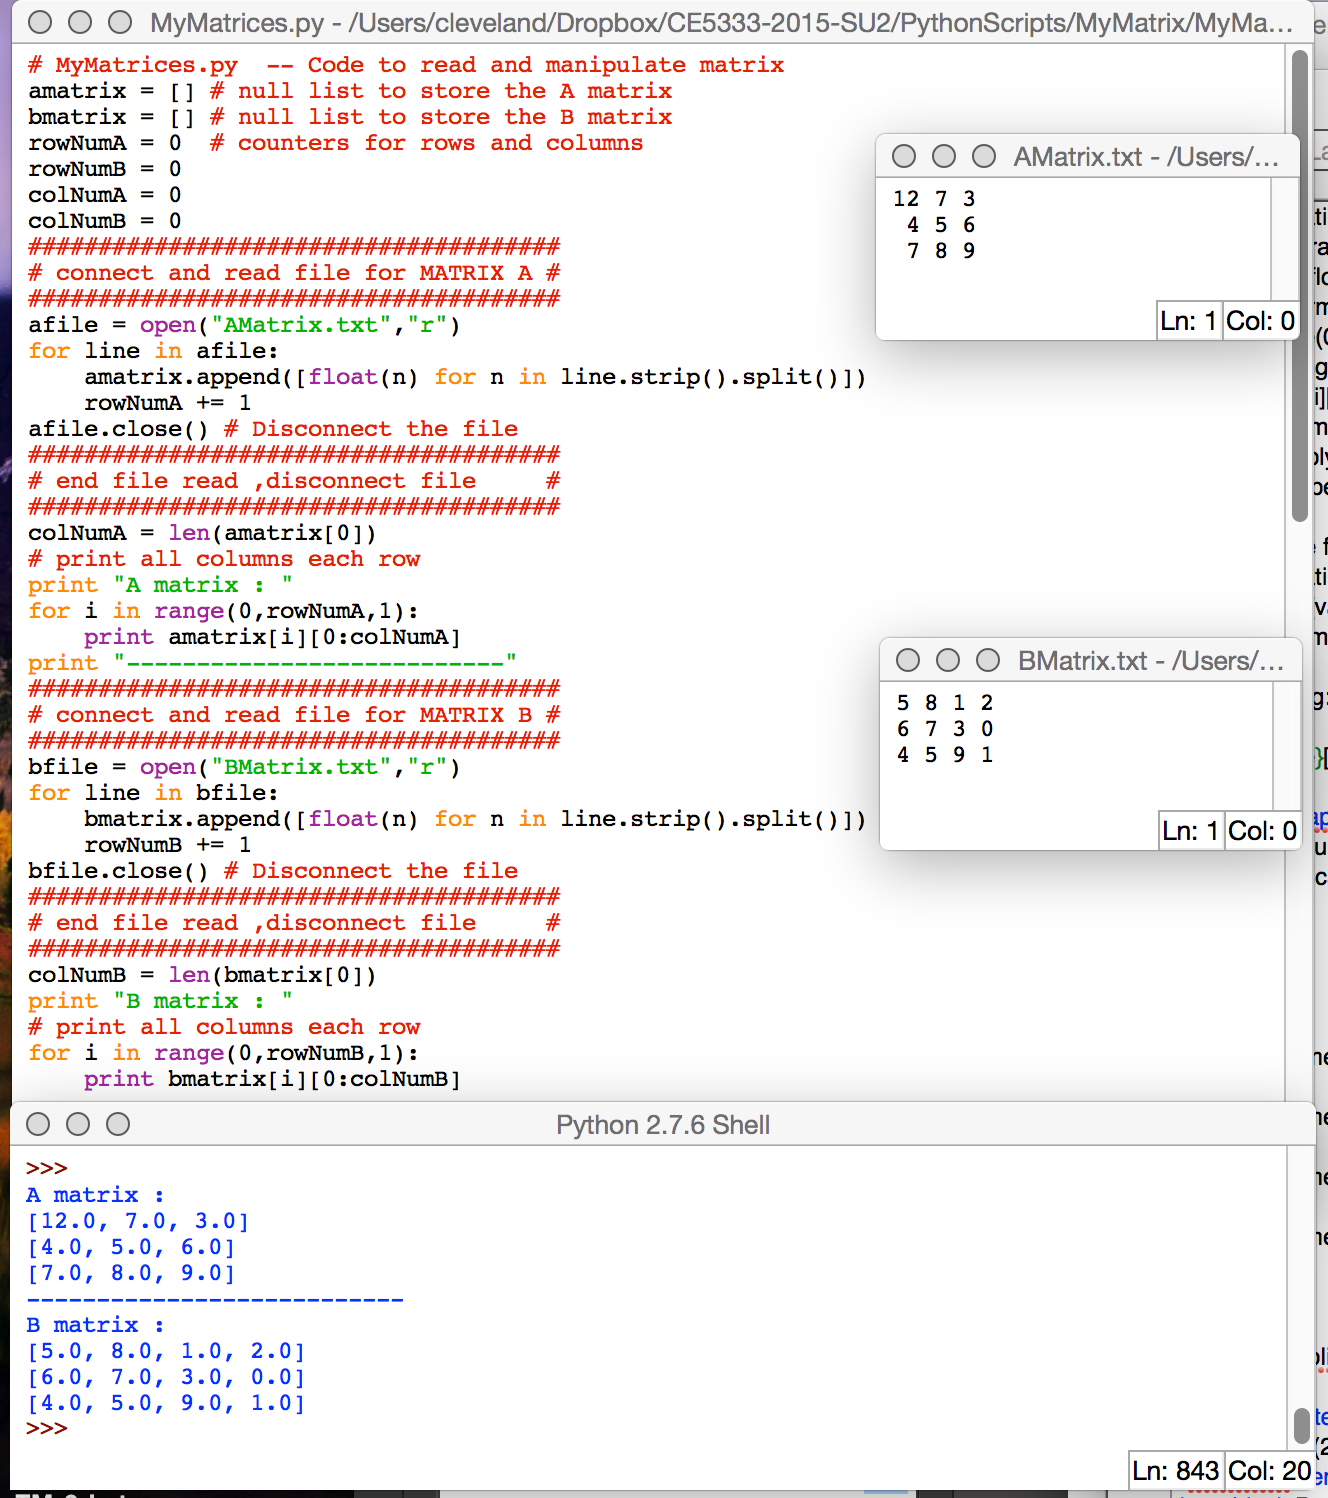
\includegraphics[width=6in]{./9-Matrix/ReadMatrixNew.jpg} 
   \caption{Reading matrix--structured data files.}
   \label{fig:ReadMatrixNew}
\end{figure}

The code itself is pretty crude -- there is no error trapping at all, but the indices are written to be adjustable as an attempt to make the code generic; with any luck we only have to write it one time (well we will write it a lot, but we only have to think hard once -- and save the code somewhere for future use.  That idea of a function library sounding better all the time!).

I am going to analyze parts of the code in the next few pages, we are into enough complication that i think such a discourse is wise.  

So here we go.  
The first part simply creates locations to read data into, null lists, and a few constants.
\begin{verbatim}
# MyMatrices.py  -- Code to read and manipulate matrix
amatrix = [] # null list to store the A matrix
bmatrix = [] # null list to store the B matrix
rowNumA = 0  # counters for rows and columns
rowNumB = 0
colNumA = 0
colNumB = 0
\end{verbatim}
\texttt{amatrix} is the name for the $\mathbf{A}$ matrix and \texttt{bmatrix} is the name for the $\mathbf{B}$ matrix.
\texttt{rowNumA} and similar names variables are going to be counters to count the number of rows and columns in each matrix.

The next part of the code opens a connection to a file that in the operating system is named \texttt{AMatrix.txt} to an object we named \texttt{afile}.
We will read lines from the file into the list variable \texttt{amatrix} as floats.
We split the string between whitespaces, and also strip excess whitespace in the \texttt{.append} method call.
We also count rows while reading the lines.  At the end of the read, we disconnect the file (close) and set the column counter to then number of things in the first row.
\begin{verbatim}
######################################
# connect and read file for MATRIX A #
######################################
afile = open("AMatrix.txt","r")
for line in afile:
    amatrix.append([float(n) for n in line.strip().split()])
    rowNumA += 1
afile.close() # Disconnect the file
######################################
# end file read ,disconnect file     #
######################################
colNumA = len(amatrix[0])
\end{verbatim}

Now the next part of the code simply writes the result back to the screen in the row-column structure we are familiar with.

\begin{verbatim}
# print all columns each row
print "A matrix : "
for i in range(0,rowNumA,1):
    print amatrix[i][0:colNumA]
print "---------------------------"   
\end{verbatim}

The trick here is that we want to write entire rows, so we use a technique called a ``slice'' where we write a portion of a list based on the first and last element in a list we wish to display.  
\texttt{print amatrix[i][0:colNumA]} is the part of the code that writes the slice of the i-th row, in this case the slice happens to be all the elements in the i-th row, but we could have chosen just a few parts or even one, or even none.

The code for the $\mathbf{B}$ matrix is identical code with just the names changed.   This is common -- we reuse code a lot.  What i illustrate here is sort of an obsolete approach.  If we have to reuse code a lot, it is to our advantage to write subroutines (or functions) that do the work so or main origami is easier to read and maintain.

\begin{verbatim}
######################################
# connect and read file for MATRIX B #
######################################
bfile = open("BMatrix.txt","r")
for line in bfile:
    bmatrix.append([float(n) for n in line.strip().split()])
    rowNumB += 1
bfile.close() # Disconnect the file
######################################
# end file read ,disconnect file     #
######################################
colNumB = len(bmatrix[0])
print "B matrix : "
# print all columns each row
for i in range(0,rowNumB,1):
    print bmatrix[i][0:colNumB]
 \end{verbatim}
 
\subsection{Matrix Arithmetic}
Now that we have a way (albeit pretty arcane) for getting matrices into our program from a file\footnote{The from a file is huge --- manually entering values will get old fast.   I have written matrix generators whose purpose in life is to construct matrices and put them into files for subsequent processing; once for a LP model the code wrote a 1200 X 1200 matrix to a file, which would be functionally impossible to enter by hand.} we can explore some elementary matrix arithmetic operations, and then will later move on to some more sophisticated operations.

Analysis of many problems in engineering result in systems of simultaneous equations.  
We typically represent systems of equations with a matrix.  
For example the two-equation system,

\begin{gather}
\begin{matrix}
2x_1 & ~+~~3x_2  \\
~\\
4x_1 & ~-~~3x_2 \\
\end{matrix}
\begin{matrix}
=~8\\
~\\
=~-2\\
\end{matrix}
\end{gather}

Could be represented by set of vectors and matrices\footnote{Usually called ``vector-matrix'' form.   Additionally, a vector is really just a matrix with column rank = 1 (a single column matrix).}

\begin{gather}
\mathbf{A} =
\begin{pmatrix}
2 & ~3 \\
~\\
4 & -3 \\
\end{pmatrix}
~
\mathbf{x} =
\begin{pmatrix}
x_1\\
~\\
x_2\\
\end{pmatrix}
~
\mathbf{b} =
\begin{pmatrix}
~8\\
~\\
-2\\
\end{pmatrix}
\end{gather}

and the linear system then written as

\begin{gather}
\mathbf{A} \cdot \mathbf{x} = \mathbf{b}
\end{gather}

So the ``algebra'' is considerably simplified, at least for writing things, 
however we now have to be able to do things like multiplication (indicated by $ ~\cdot $) as well as the concept of addition and subtraction, and division (multiplication by an inverse).  
There are also several kinds of matrix multiplication -- the inner product as required by the linear system, the vector (cross product), the exterior (wedge), and outer (tensor) product are a few of importance in both mathematics and engineering. 

The remainder of this section will examine the more common matrix operations.
\subsubsection{Matrix Definition}
A matrix is a rectangular array of numbers.
\begin{gather}
\begin{pmatrix}
1 & 5 & 7 & 2\\
2 & 9 & 17 & 5 \\
11 & 15 & 8 & 3 \\
\end{pmatrix}
\end{gather}

The size of a matrix is referred to in terms of the number of rows and the number of columns.  The enclosing parenthesis are optional above, but become meaningful when writing multiple matrices next to each other.
The above matrix is 3 by 4.  

When we are discussing matrices we will often refer to specific numbers in the matrix.  
To refer to a specific element of a matrix we refer to the row number (i) and the column number (j).  
We will often call a specific element of the matrix, the $a_{i,j}$ -th element of the matrix.  For example $a_{2,3}$ element in the above matrix is 17.  We have seen in Python that we would refer to the element as \texttt{a\_matrix[i][j]} or whatever the name of the matrix is in the program.

\subsubsection{Multiply a matrix by a scalar}
A scalar multiple of a matrix is simply each element of the matrix multiplied by the scalar value.
 Consider the matrix $\mathbf{A}$ below.
\begin{gather}
\mathbf{A}=
\begin{pmatrix}
1 & 5 & 7 \\
2 & 9 & 3 \\
4 & 4 & 8 \\
\end{pmatrix}
\end{gather}

If the scalar is say 2, then $2 \times \mathbf{A}$ is computed by doubling each element of $\mathbf{A}$, as

\begin{gather}
2\mathbf{A}=
\begin{pmatrix}
2 & 10 & 14\\
4 & 18 & 6 \\
8 & 8 & 16 \\
\end{pmatrix}
\end{gather}

In Python we can simply perform the element-by-element arithmetic

\begin{verbatim}
MyScalar = raw_input("Enter scalar value for multiply matrix \n")
MyScalar = float(MyScalar)  # force a float
# now perform element-by-element multiplication
for i in range(0,rowNumA,1):
   for j in range(0,colNumA,1):
       amatrix[i][j] = MyScalar * amatrix[i][j]
\end{verbatim}


Figure \ref{fig:ScalarMultiply} is an example using the earlier $\mathbf{A}$ matrix and multiplying it by the scalar value of 2.0.   
We did the beginning of a rudimentary error trap to force the scalar to be a real number before performing the multiplication.

\begin{figure}[h!] %  figure placement: here, top, bottom, or page
   \centering
   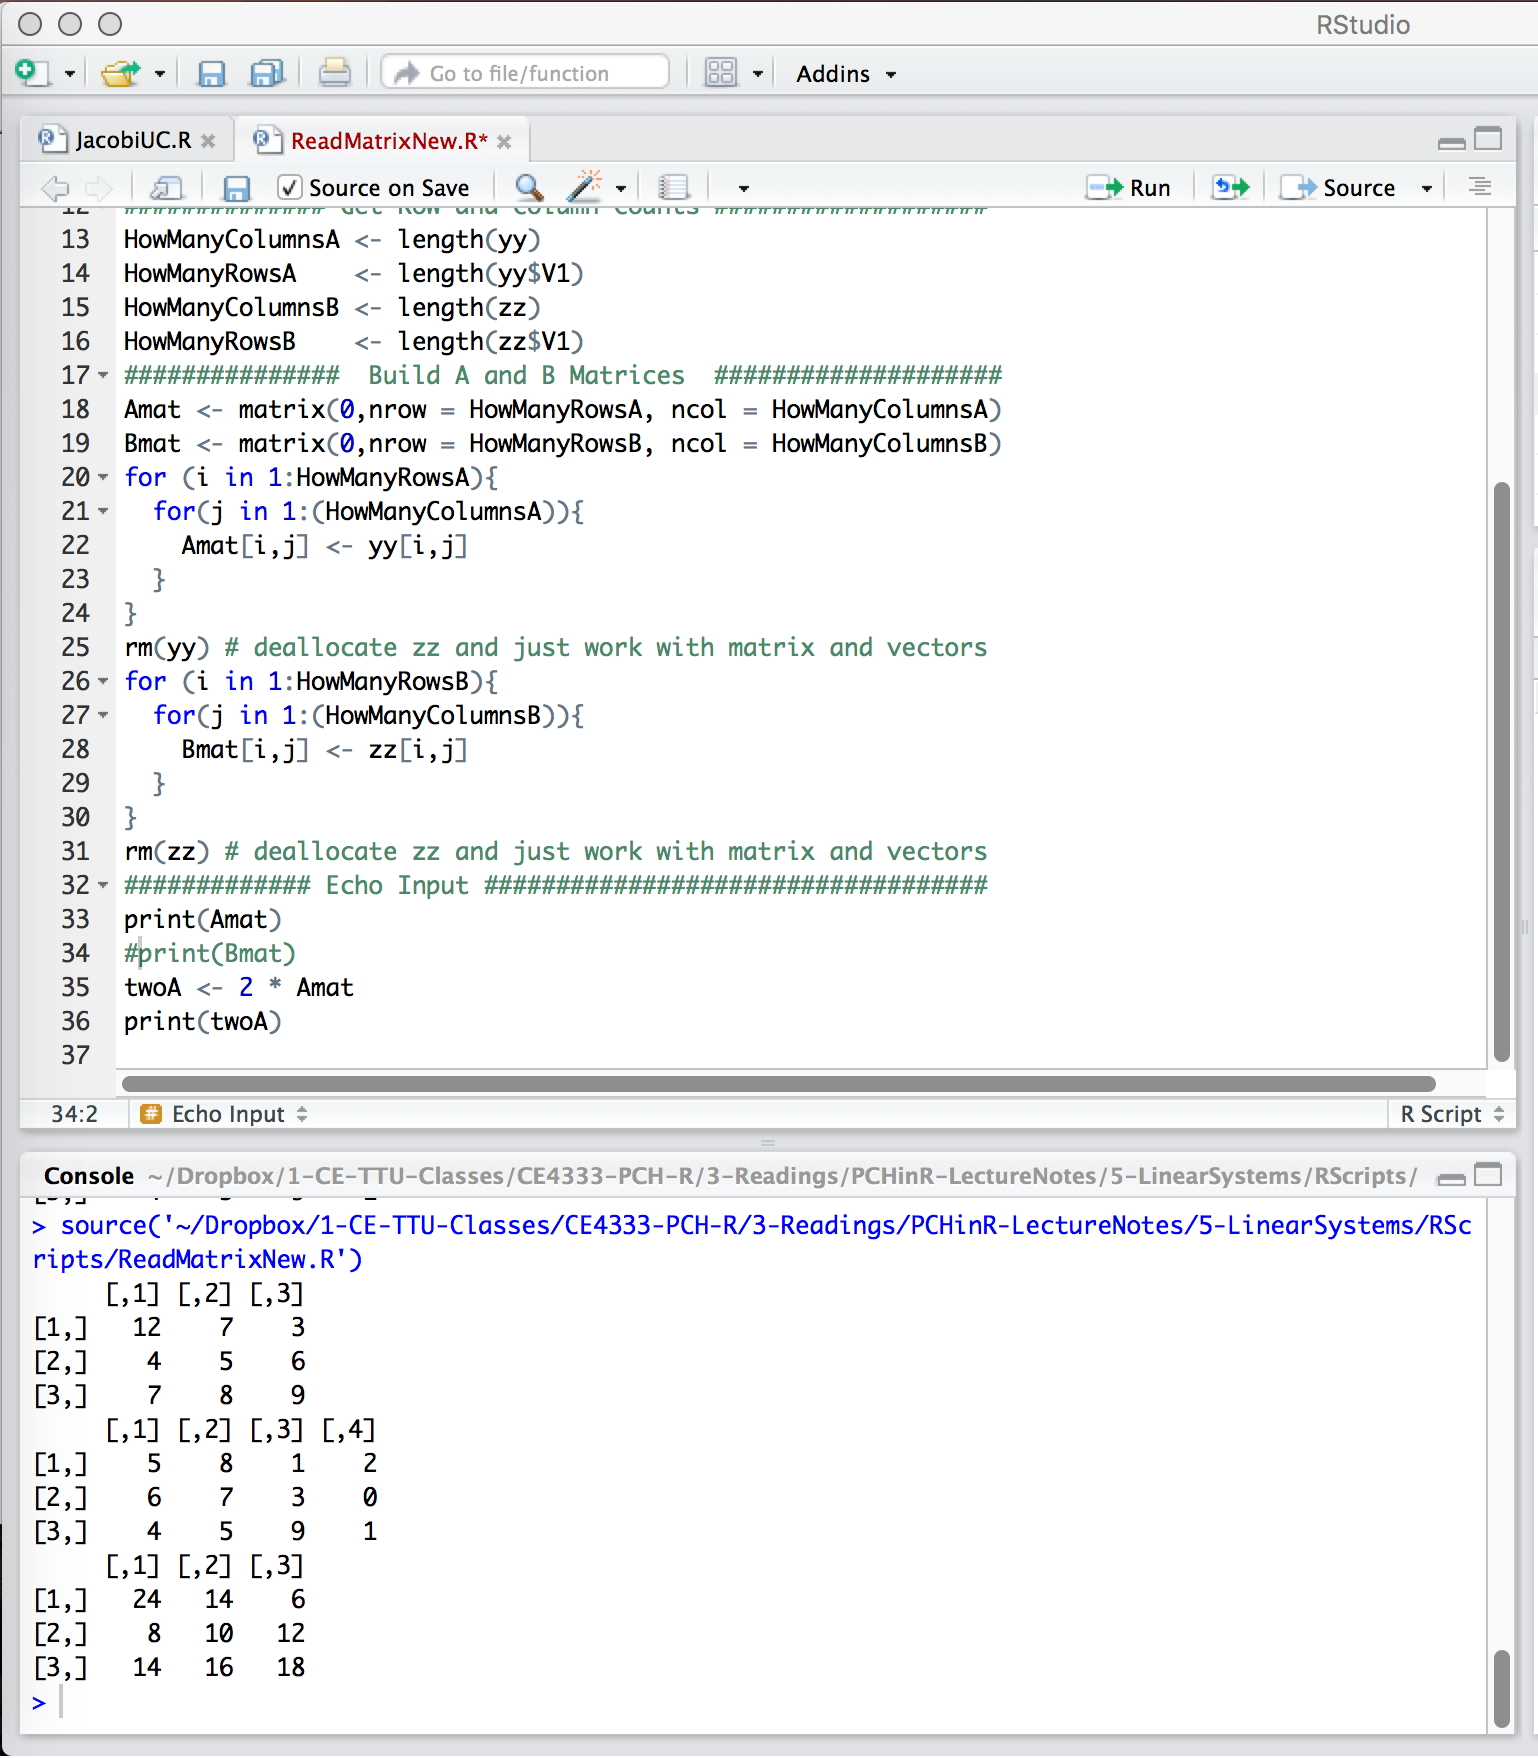
\includegraphics[width=6in]{./9-Matrix/ScalarMultiply.jpg} 
   \caption{Multiply each element in \texttt{amatrix} by a scalar }
   \label{fig:ScalarMultiply}
\end{figure}

\clearpage
 \subsubsection{Matrix addition (and subtraction)}
Matrix addition and subtraction are also element-by-element operations.
In order to add or subtract two matrices they must be the same size and shape.  
This requirement means that they must have the same number of rows and columns.  
To add or subtract a matrix we simply add or subtract the corresponding elements from each matrix.

For example consider the two matrices $\mathbf{A}$ and $\mathbf{B}$ below

\begin{gather}
\mathbf{A}=
\begin{pmatrix}
1 & 5 & 7 \\
2 & 9 & 3 \\
\end{pmatrix}
~ 
\mathbf{B}=
\begin{pmatrix}
3 & -2 & 1 \\
-2 & 1 & 1 \\
\end{pmatrix}
\end{gather}

For example the sum of these two matrices is the matrix named $\mathbf{A+B}$,  shown below:

\begin{gather}
\mathbf{A+B}=
\begin{pmatrix}
1+3 & 5-2 & 7+1 \\
2-2 & 9+1 & 3+1 \\
\end{pmatrix}
=
\begin{pmatrix}
4 & 3 & 8 \\
0 & 10 & 4 \\
\end{pmatrix}
\end{gather}

Now to do the operation in Python, we need to read in the matrices, perform the addition, and write the result.  
In the code example in \ref{fig:AddMatrix} I added a third matrix to store the result -- generally we don't want to clobber existing matrices, so we will use the result instead.   

Also notice the construction of the third matrix, because I should know the size I can use a double iterator assignment to create and fill the matrix with zeros in the correct size and shape.  

\begin{figure}[h!] %  figure placement: here, top, bottom, or page
   \centering
   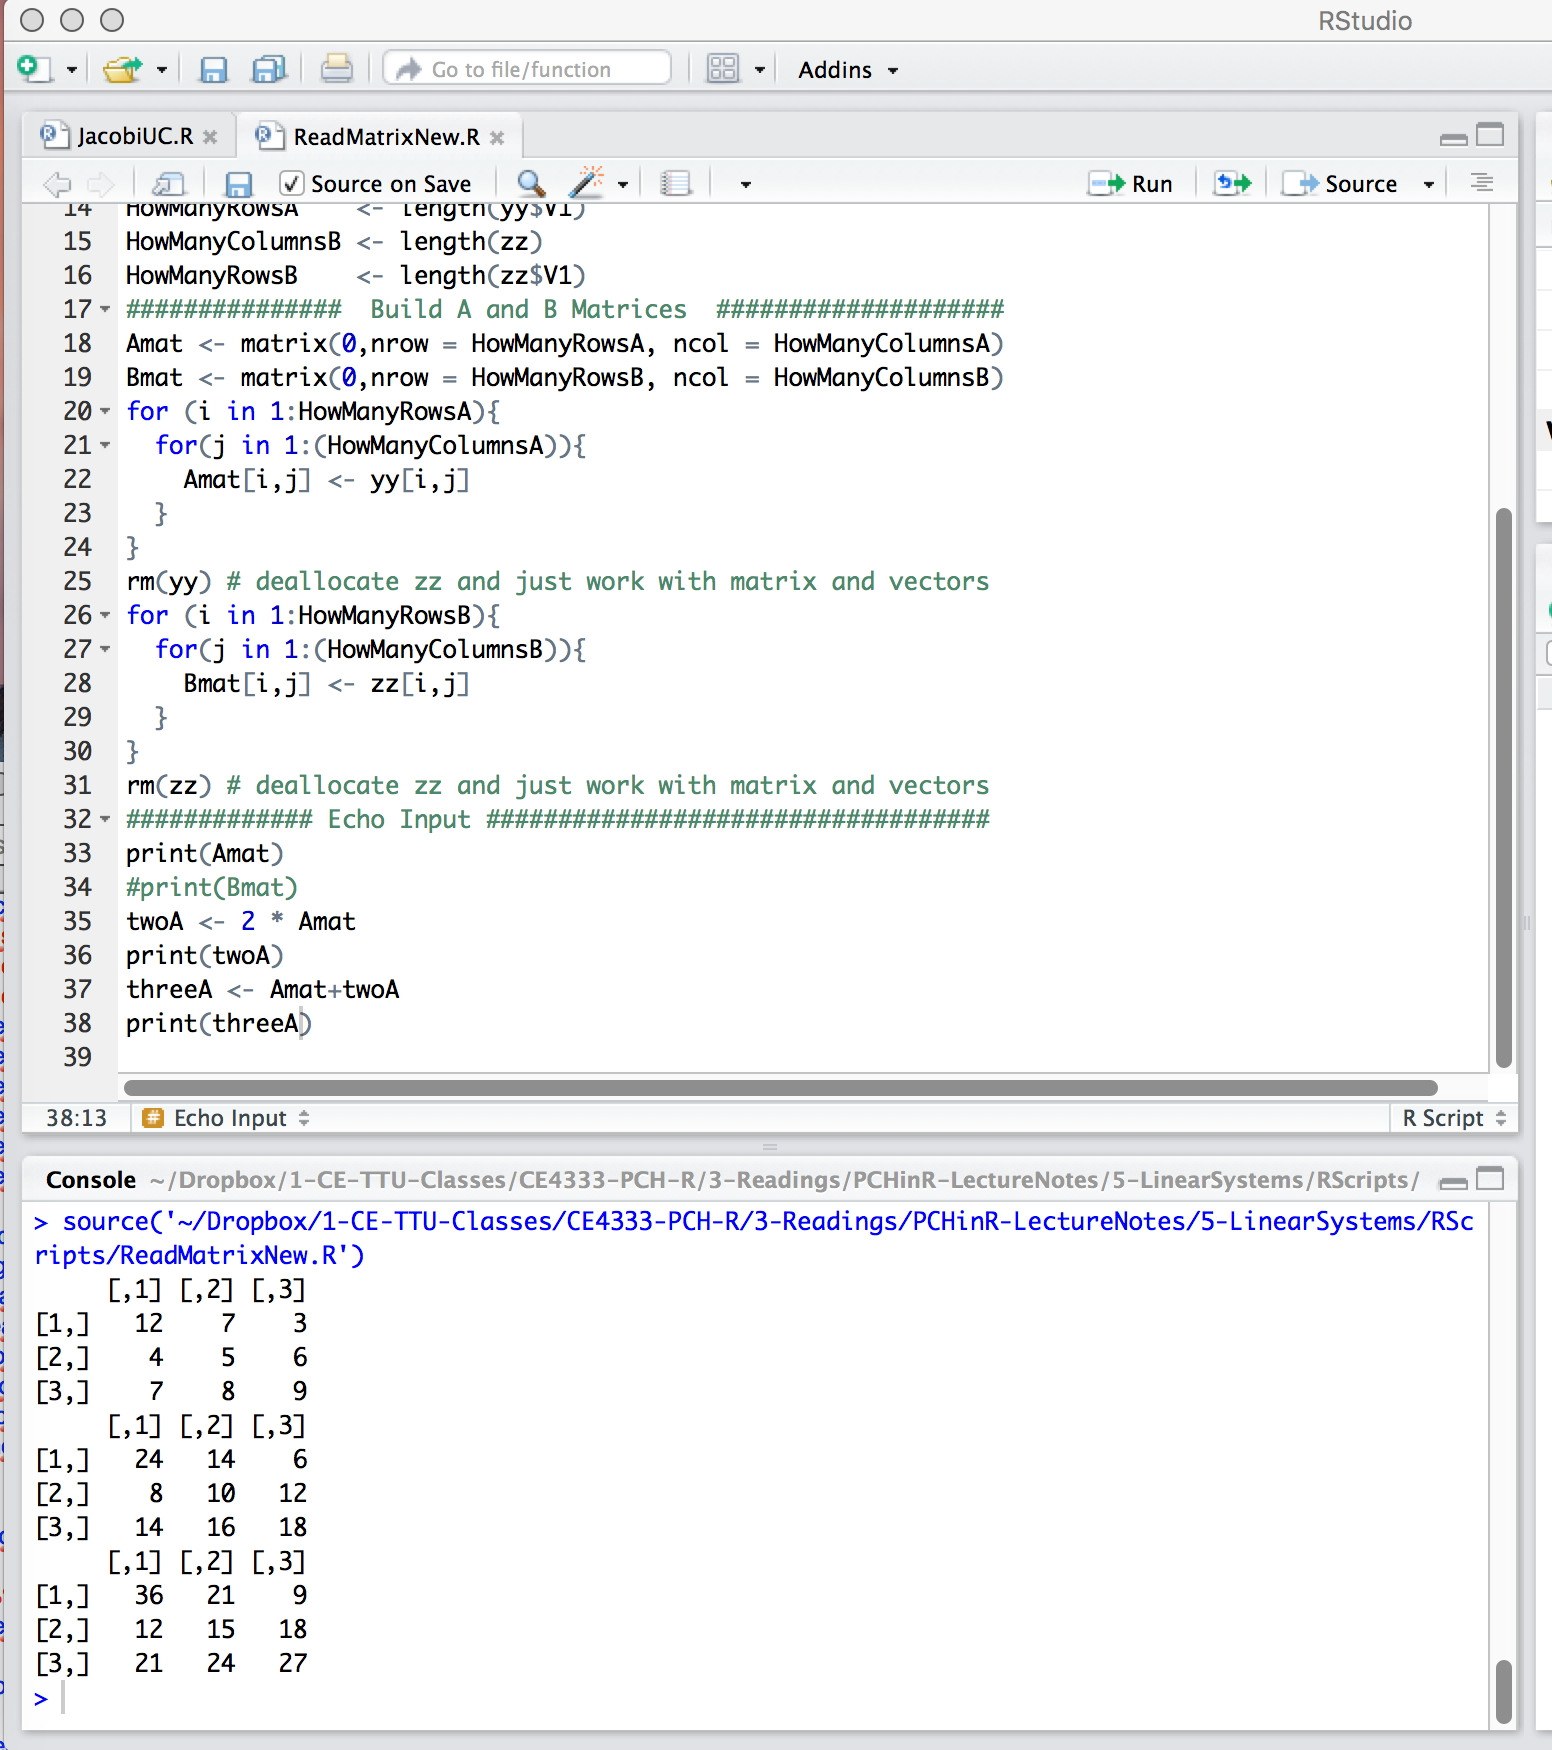
\includegraphics[width=6in]{./9-Matrix/AddMatrix.jpg} 
   \caption{Add each element in \texttt{amatrix} to each element in \texttt{bmatrix}, store the result in \texttt{result\_matrix}.}
   \label{fig:AddMatrix}
\end{figure}

Subtraction is performed in a similar fashion, except the subtraction operator is used.  
\clearpage
\subsubsection{Multiply a matrix}
One kind of matrix multiplication is an inner product.  
Usually when matrix multiplication is mentioned without further qualification ,the implied meaning is an inner product of the matrix and a vector (or another matrix).

Matrix multiplication is  more complex than addition and subtraction.  
If two matrices such as a matrix $\mathbf{A}$ (size l x m) and a matrix $\mathbf{B}$ ( size m x n) are multiplied together, the resulting matrix $\mathbf{C}$ has a size of l x n.  
The order of multiplication of matrices is extremely important\footnote{Matrix multiplication is not  transitive;  $\mathbf{A}~\mathbf{B} ~\ne~  \mathbf{B}~\mathbf{A}$.}.  

To obtain $\mathbf{C}$ = $\mathbf{A}$ $\mathbf{B}$, the number of columns in $\mathbf{A}$ must be the same as the number of rows in $\mathbf{B}$.  In order to carry out the matrix operations for multiplication of matrices, the $i,j$-th element of  $\mathbf{C}$ is simply equal to the scalar (dot or inner) product of row $i$ of $\mathbf{A}$ and column $j$ of $\mathbf{B}$.

Consider the example below
\begin{gather}
\mathbf{A}=
\begin{pmatrix}
1 & 5 & 7 \\
2 & 9 & 3 \\
\end{pmatrix}
~ 
\mathbf{B}=
\begin{pmatrix}
3 & -2  \\
-2 & 1 \\
1 & 1 \\
\end{pmatrix}
\end{gather}

First, we would evaluate if the operation is even possible, $\mathbf{A}$ has two rows and three columns.  
$\mathbf{B}$ has three rows and two columns.  
By our implied multiplication ``rules'' for the multiplication to be defined the first matrix must have the same number of rows as the second matrix has columns (in this case it does), and the result matrix will have the same number of rows as the first matrix, and the same number of columns as the second matrix (in this case the result will be a 2X2 matrix).

\begin{gather}
\mathbf{C}=\mathbf{A}\mathbf{B}=
\begin{pmatrix}
c_{1,1} & c_{1,2} \\
c_{2,1} & c_{2,2} \\
\end{pmatrix}
\end{gather}

And each element of $\mathbf{C}$ is the dot product of the row vector of $\mathbf{A}$ and the column vector of $\mathbf{B}$.
\newpage

\begin{gather}
c_{1,1} =
\begin{pmatrix}
1 & 5 & 7 \\
\end{pmatrix}
\cdot
\begin{pmatrix}
3 \\
-2 \\
1 \\
\end{pmatrix}
=
\begin{pmatrix}
(1)(3) +(5)(-2) + (7)(1)\\
\end{pmatrix}
= 0
\end{gather}

\begin{gather}
c_{1,2} =
\begin{pmatrix}
1 & 5 & 7 \\
\end{pmatrix}
\cdot
\begin{pmatrix}
-2 \\
1 \\
1 \\
\end{pmatrix}
=
\begin{pmatrix}
(1)(-2) +(5)(1) + (7)(1)\\
\end{pmatrix}
= 10
\end{gather}


\begin{gather}
c_{2,1} =
\begin{pmatrix}
2 & 9 & 3 \\
\end{pmatrix}
\cdot
\begin{pmatrix}
3 \\
-2 \\
1 \\
\end{pmatrix}
=
\begin{pmatrix}
(2)(3) +(9)(-2) + (3)(1)\\
\end{pmatrix}
= -9
\end{gather}


\begin{gather}
c_{2,2} =
\begin{pmatrix}
2 & 9 & 3 \\
\end{pmatrix}
\cdot
\begin{pmatrix}
-2 \\
1 \\
1 \\
\end{pmatrix}
=
\begin{pmatrix}
(2)(-2) +(9)(1) + (3)(1)\\
\end{pmatrix}
= 8
\end{gather}

Making the substitutions results in :

\begin{gather}
\mathbf{C}=\mathbf{A}\mathbf{B}=
\begin{pmatrix}
0 & 10 \\
-9 & 8 \\
\end{pmatrix}
\end{gather}

So in an algorithmic sense we will have to deal with three matrices, the two source matrices and the destination matrix.  
We will also have to manage element-by-element multiplication and be able to correctly store through rows and columns.

Figure \ref{fig:MultiplyMatrix} is a script that multiplies the two matrices above and prints the result.   
The actual code for the multiplication is three nested for-loops.  
The outer loop counts based rows of the first matrix, the middle loop counts based on columns of the second matrix, and the inner most loop counts based on columns of the first matrix ( or rows of the second matrix).   

Because we initialized the result matrix with zeros before starting the operation we can use it as the accumulator for the element-by-element multiplication.

\begin{figure}[h!] %  figure placement: here, top, bottom, or page
   \centering
   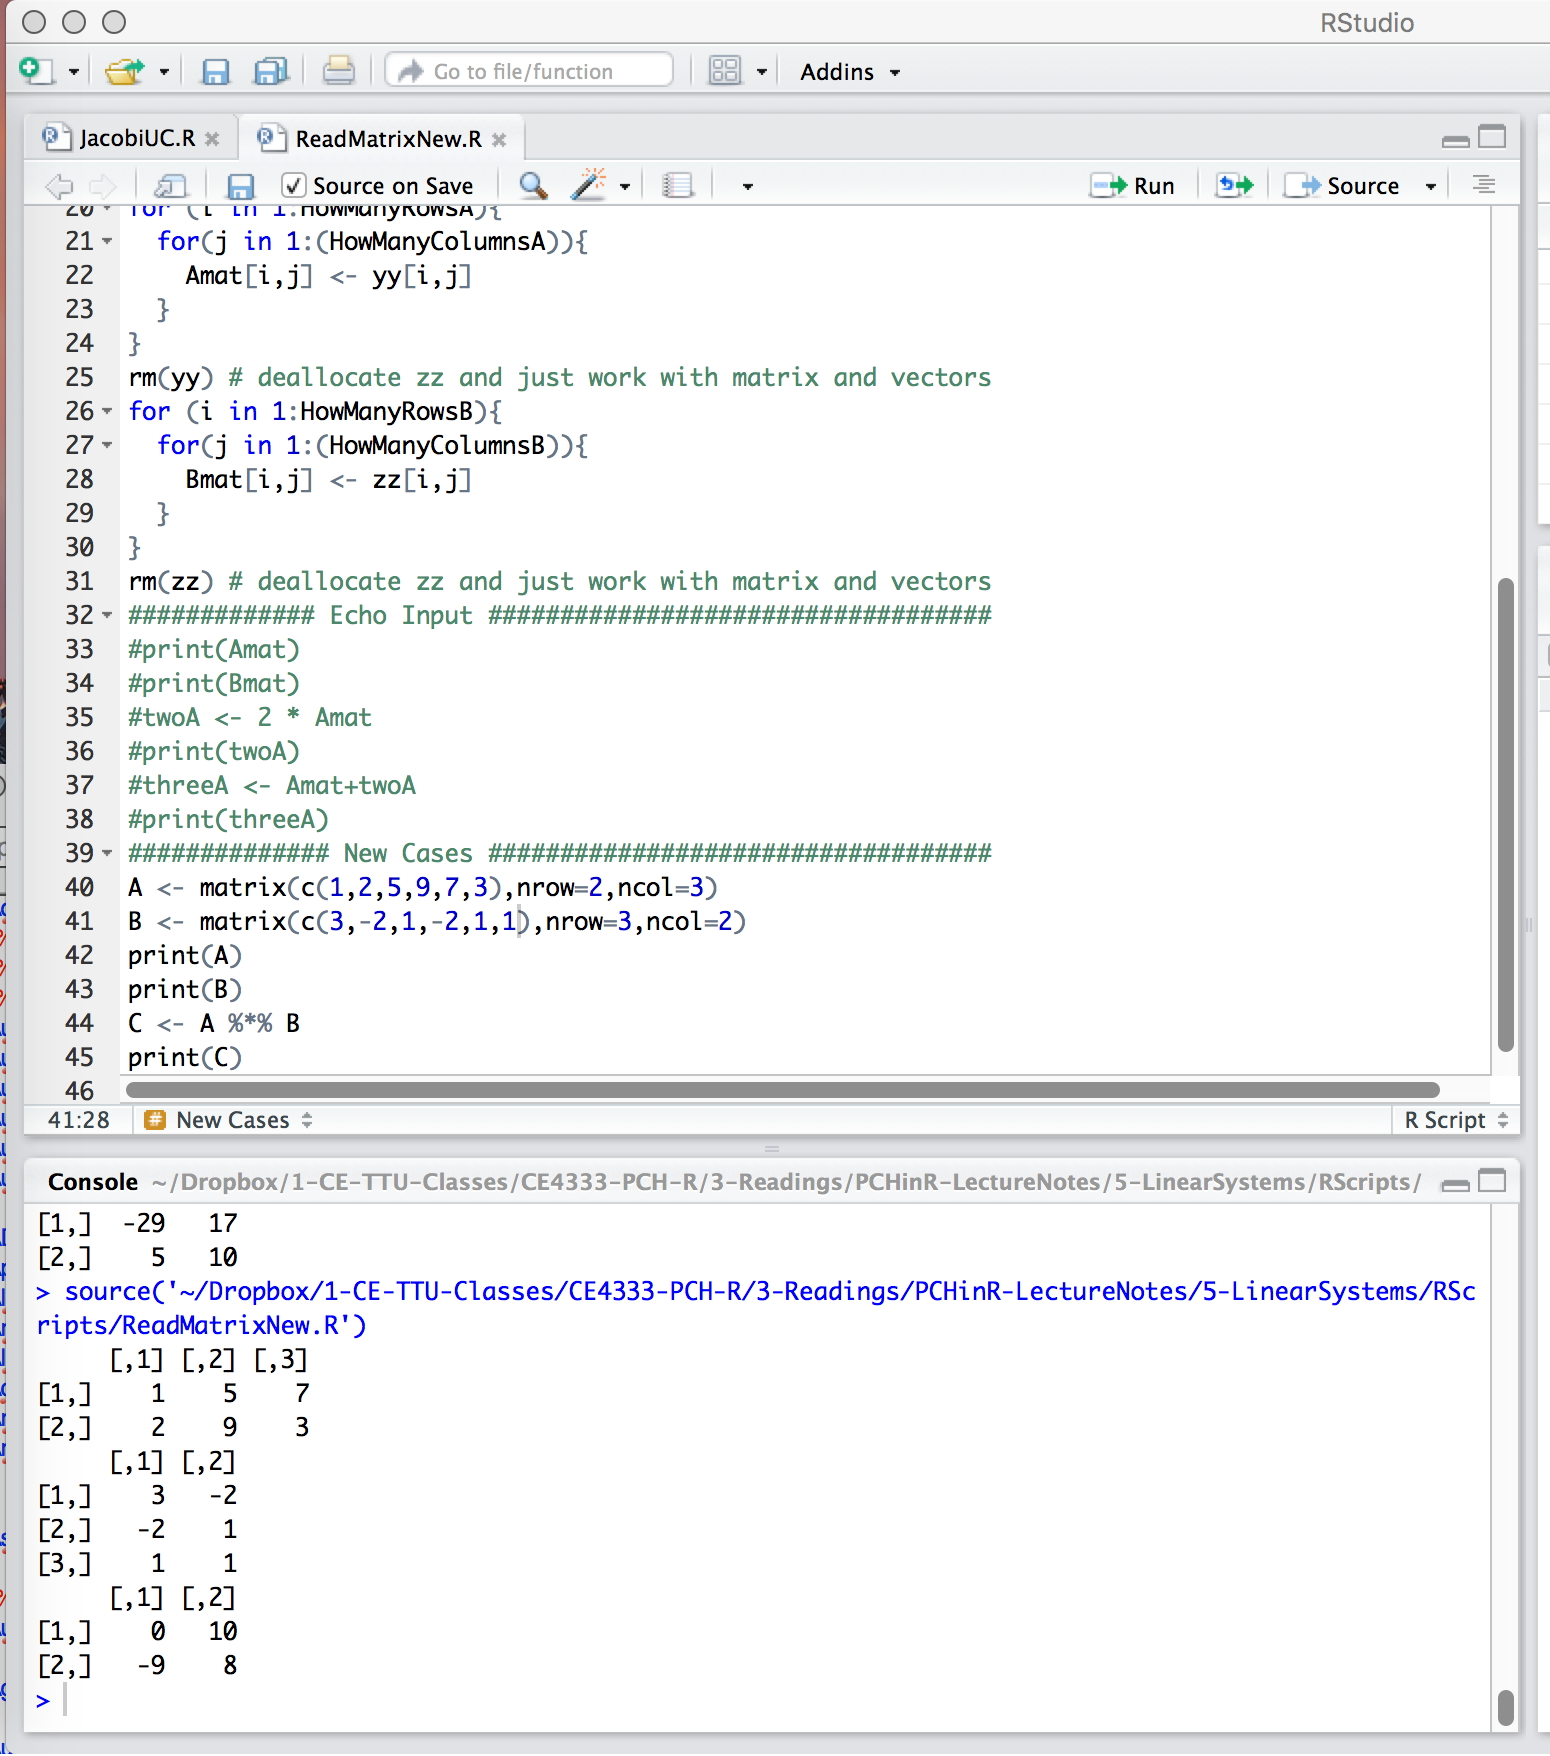
\includegraphics[width=6in]{./9-Matrix/MultiplyMatrix.jpg} 
   \caption{Matrix multiplication example}
   \label{fig:MultiplyMatrix}
\end{figure}
\clearpage
\subsubsection{Identity matrix}
In computational linear algebra we often need to make use of a special matrix called the ``Identity Matrix''.  
The Identity Matrix is a square matrix with all zeros except the $i,i$0-th element (diagonal) which is equal to 1:

\begin{gather}
\mathbf{I}_{3\times3}=
\begin{pmatrix}
1 & 0 & 0\\
0 & 1 & 0\\
0 & 0 & 1\\
\end{pmatrix}
\end{gather}
Usually we don't bother with the size subscript i used above and just stipulate that the matrix is sized as appropriate.
Multiplying any matrix by (a correctly sized) identity matrix results in no change in the matrix.  $\mathbf{I}\mathbf{A} = \mathbf{A}$  

\subsubsection{Matrix Inverse}
In many practical computational and theoretical operations we employ the concept of the inverse of a matrix.
The inverse is somewhat analogous to``dividing'' by the matrix.  
Consider our linear system 
\begin{gather}
\mathbf{A} \cdot \mathbf{x} = \mathbf{b}
\end{gather}
If we wished to solve for $\mathbf{x}$ we would ``divide'' both sides of the equation by $\mathbf{A}$.   
Instead of division (which is essentially left undefined for matrices) we instead multiply by the inverse of the matrix\footnote{The matrix inverse is the multiplicative inverse of the matrix -- we are defining a division operation, just calling it something else.}.
The inverse of a matrix $\mathbf{A}$ is denoted by $\mathbf{A}^{-1}$ and by definition is a matrix such that when $\mathbf{A}^{-1}$ and $\mathbf{A}$ are multiplied together, the identity matrix $\mathbf{I}$ results.  e.g. $\mathbf{A}^{-1} \mathbf{A} = \mathbf{I}$

Lets consider the matrixes below
\begin{gather}
\mathbf{A}=
\begin{pmatrix}
2 & 3 \\
4 & -3 \\
\end{pmatrix}
\end{gather}

\begin{gather}
\mathbf{A}^{-1}=
\begin{pmatrix}
\frac{1}{6} & \frac{1}{6} \\
~\\
\frac{2}{9} & -\frac{1}{9} \\
\end{pmatrix}
\end{gather}

We can check that the matrices are indeed inverses of each other using our Python code.  
Figure \ref{fig:InverseMatrixCheck} is our multiplication script modified to read the $\mathbf{A}$ and $\mathbf{A}^{-1}$
perform the multiplication and then report the result.   
The result is the identity matrix regardless of the order of operation.\footnote{Why do you think this is so, when above we stated that multiplication is intransitive?}

\begin{figure}[h!] %  figure placement: here, top, bottom, or page
   \centering
   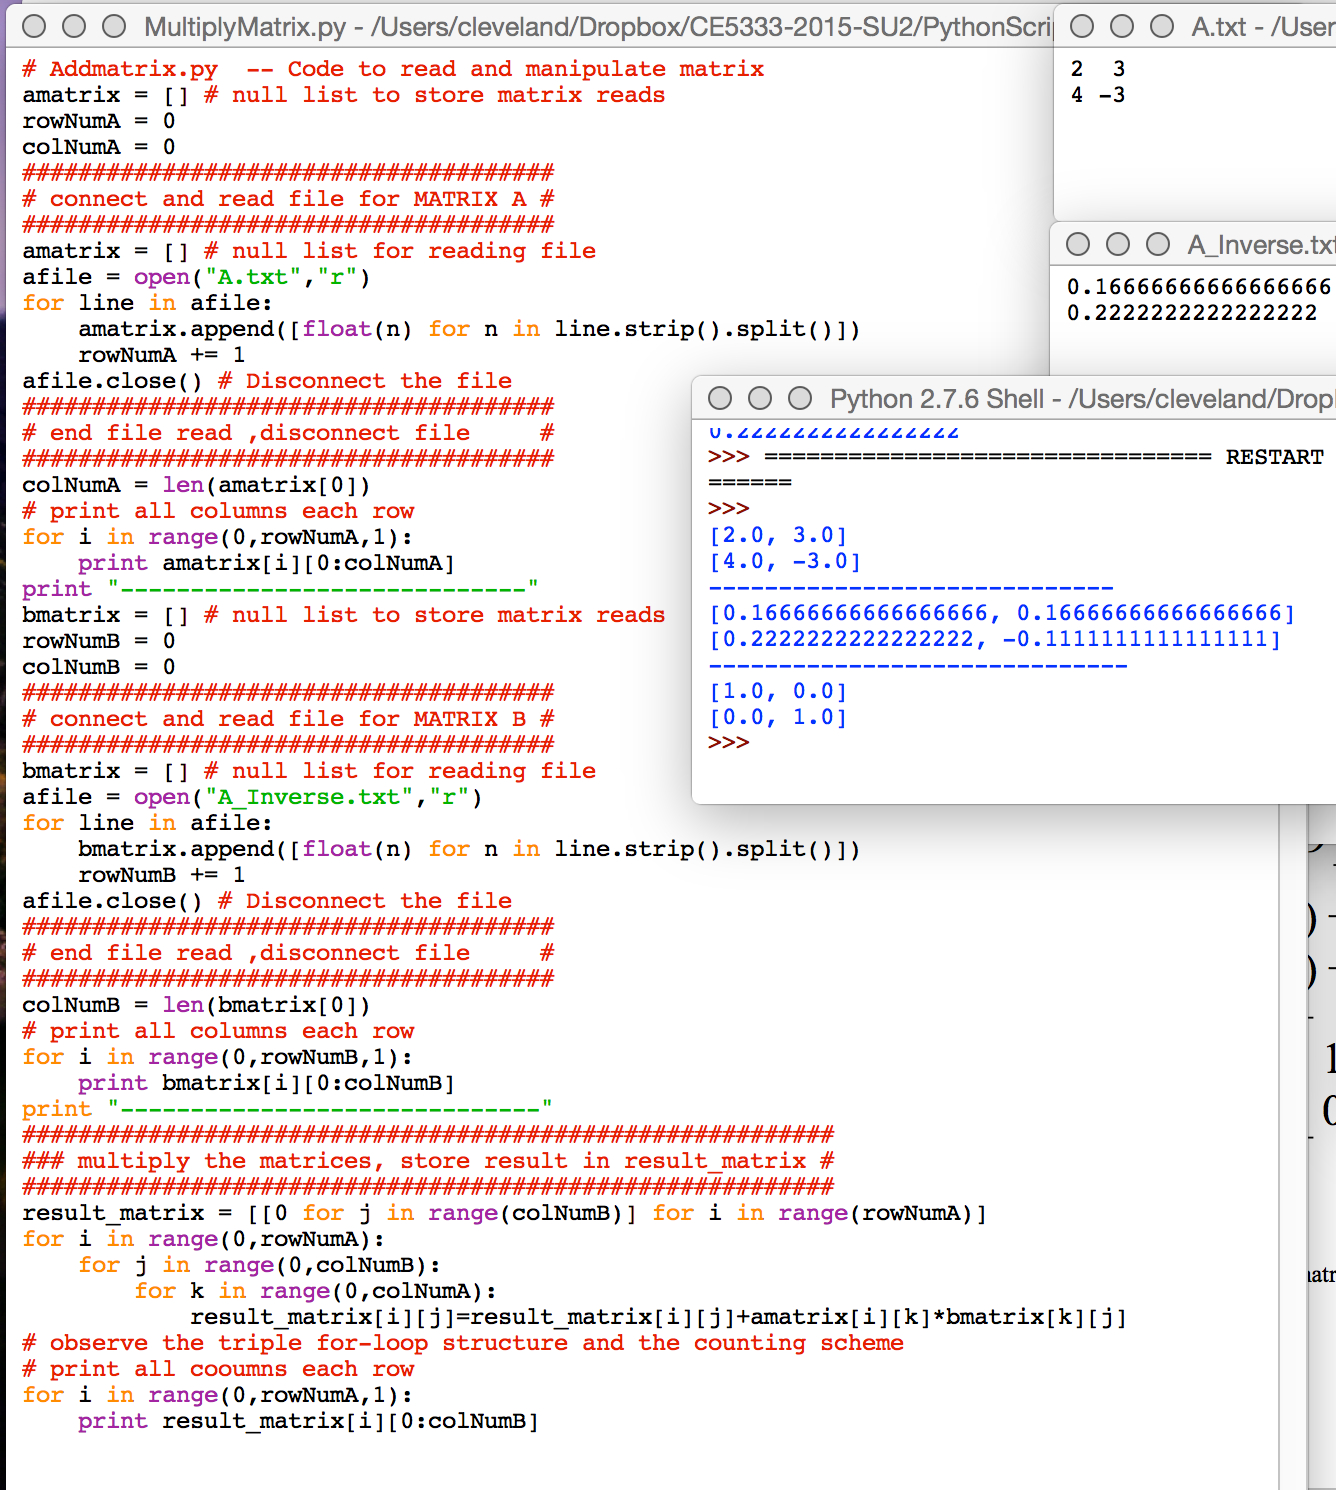
\includegraphics[width=5in]{./9-Matrix/InverseMatrixCheck.jpg} 
   \caption{Matrix multiplication used to check an inverse.}
   \label{fig:InverseMatrixCheck}
\end{figure}
\clearpage

Now that we have some background on what an inverse is, it would be nice to know how to find them --- that is a remarkably challenging problem.   Here we examine a classical algorithm for finding an inverse if we really need to --- computationally we only invert if necessary, there are other ways to ``divide'' that are faster.

\subsubsection{Gauss-Jordan method of finding $\mathbf{A}^{-1}$}
There are a number of methods that can be used to find the inverse of a matrix using elementary row operations.  
An elementary row operation is any one of the three operations listed below:
\begin{enumerate}
\item Multiply or divide an entire row by a constant.
\item Add or subtract a multiple of one row to/from another.
\item Exchange the position of any 2 rows.
\end{enumerate}

The Gauss-Jordan method of inverting a matrix can be divided into 4 main steps.  
In order to find the inverse we will be working with the original matrix, augmented with the identity matrix -- this new matrix is called the augmented matrix (because no-one has tried to think of a cooler name yet).  

\begin{gather}
\mathbf{A} | \mathbf{I} =
\begin{pmatrix}
2 & 3 & | & 1 & 0 \\
4 & -3 & | & 0 & 1 \\
\end{pmatrix}
\end{gather}

We will perform elementary row operations based on the left matrix to convert it to an identity matrix -- we perform the same operations on the right matrix and the result when we are done is the inverse of the original matrix.

So here goes -- in the theory here, we also get to do infinite-precision arithmetic, no rounding/truncation errors.  

\begin{enumerate}
\item Divide row one by the $a_{1,1}$ value to force a $1$ in the $a_{1,1}$ position.   This is elementary row operation 1 in our list above.
\begin{gather}
\mathbf{A} | \mathbf{I} =
\begin{pmatrix}
2/2 & 3/2 & | & 1/2 & 0 \\
4 & -3 & | & 0 & 1 \\
\end{pmatrix}
=
\begin{pmatrix}
1 & 3/2 & | & 1/2 & 0 \\
4 & -3 & | & 0 & 1 \\
\end{pmatrix}
\end{gather}

\item For all rows below the first row, replace $row_j$ with $row_j - a_{j,1}*row_1$.  
This happens to be elementary row operation 2 in our list above.
\begin{gather}
\mathbf{A} | \mathbf{I} =
\begin{pmatrix}
1 & 3/2 & | & 1/2 & 0 \\
4 - 4(1) & -3 - 4(3/2) & | & 0-4(1/2) & 1-4(0) \\
\end{pmatrix}
=
\begin{pmatrix}
1 & 3/2 & | & 1/2 & 0 \\
0 & -9 & | & -2 & 1 \\
\end{pmatrix}
\end{gather}


\item Now multiply $row_2$ by $ \frac{1}{ a_{2,2}} $.  This is again elementary row operation 1 in our list above.

\begin{gather}
\mathbf{A} | \mathbf{I} =
\begin{pmatrix}
1 & 3/2 & | & 1/2 & 0 \\
0 & -9/-9 & | & -2/-9 & 1/-9 \\
\end{pmatrix}
=
\begin{pmatrix}
1 & 3/2 & | & 1/2 & 0 \\
0 & 1 & | & 2/9 & -1/9 \\
\end{pmatrix}
\end{gather}

\item For all rows above and below this current row, replace $row_j$ with $row_j - a_{2,2}*row_2$.  
This happens to again be elementary row operation 2 in our list above.  
What we are doing is systematically converting the left matrix into an identity matrix by multiplication of constants and addition to eliminate off-diagonal values and force 1 on the diagonal.

\begin{gather}
\mathbf{A} | \mathbf{I} = \\
\begin{pmatrix}
1 & 3/2 - (3/2)(1) & | & 1/2 - (3/2)(2/9) & 0-(3/2)(-1/9) \\
0 & 1 & | & 2/9 & -1/9 \\
\end{pmatrix}
= \\
\begin{pmatrix}
1 & 0 & | & 1/6 & 1/6 \\
0 & 1 & | & 2/9 & -1/9 \\
\end{pmatrix}
\end{gather}

\item As far as this example is concerned we are done and have found the inverse.  
With more than a 2X2 system there will be many operations moving up and down the matrix to eliminate the off-diagonal terms.
\end{enumerate}

So the next logical step is to build an algorithm to perform these operations for us.

The code for inversion is a bit long, so it is first recorded here as a script (by parts), then multiple screen captures.

The first part (next page) reads in the matrix from a file named ``A.txt'', and then builds some workspaces for the inversion process.
One of the workspaces is a matrix called ``bmatrix'' which is an identity matrix and is also the augmented portion of the system depicted in the 2X2 example.  The actual inverse gets stored in a matrix named ``xmatrix'', which is really a column-by-column collection of solutions to a linear system where the right hand side is the different columns of the identity matrix. 
 
\newpage
\begin{verbatim}
# InvertASystem.py
# Code to read A matrix, then invert the matrix by
# repeated solve of Ax = b for x by Gaussian elimination with back substitution
# where b is a vector (column) from an identity matrix
#
print "Matrix Inversion"
amatrix = [] # null list to store matrix reads
rowNumA = 0
colNumA = 0
#
# connect and read the A-matrix from a file
#
afile = open("A.txt","r")
for line in afile:
    amatrix.append([float(n) for n in line.strip().split()])
    rowNumA += 1
colNumA = len(amatrix[0])
#
# disconnect the file
#
afile.close()
#
# workspaces for the numerical linear algebra
#
bmatrix = [[0 for j in range(colNumA)]for i in range(rowNumA)]
cmatrix = [[0 for j in range(colNumA)]for i in range(rowNumA)]
dmatrix = [[0 for j in range(colNumA)]for i in range(rowNumA)]
xmatrix = [[0 for j in range(colNumA)]for i in range(rowNumA)]
#
# build bmatrix into an identity matrix
#
for i in range(0,rowNumA,1):
    bmatrix[i][i] = 1.0
#
# copy amatrix into dmatrix  -- this is a static copy
#
dmatrix = [[amatrix[i][j] for j in range(colNumA)]for i in range(rowNumA)]
\end{verbatim}

Now we have set up the workspaces, initialized them (filled them with zeros and ones as appropriate), next we step through the inversion process.  The algorithm used here is crude and destroys the coefficient matrix each time it is invoked, so we need to keep a copy of the original matrix.   I chose to use the ``dmatrix'' for this use --- it is never changed, but is used to rebuild the coefficient matrix and an intermediate matrix for each different right hand side.

The next part performs the actual inversion.

\begin{verbatim}
#
# now attempt inversion
#
# outer wrapper loop
#
for jcol in range(rowNumA):
#
# reset the amatrix and cmatrix for this column bmatrix
#
    amatrix = [[dmatrix[i][j] for j in range(colNumA)]for i in range(rowNumA)]
    cmatrix = [[dmatrix[i][j] for j in range(colNumA)]for i in range(rowNumA)]
# build the diagonal -- assume diagonally dominant
    for k in range(rowNumA-1):
        l = k+1
        for i in range(l,rowNumA):
            for j in range(colNumA):
                cmatrix[i][j]=amatrix[i][j]-amatrix[k][j]*amatrix[i][k]/amatrix[k][k]
            bmatrix[i][jcol] = bmatrix[i][jcol]-bmatrix[k][jcol]*amatrix[i][k]/amatrix[k][k]
        for i in range(rowNumA):
            for j in range(colNumA):
                amatrix[i][j] = cmatrix[i][j]
#
# gaussian reduction this column of bmatrix done
#
# now for the back substitution
#
    for k in range(rowNumA-1,-1,-1):
        sum1 = 0.0
        for i in range(rowNumA):
            if i == k:
                continue 
            else:
                sum1 = sum1 + amatrix[k][i]*xmatrix[i][jcol]
            xmatrix[k][jcol]=(bmatrix[k][jcol] - sum1)/amatrix[k][k]
\end{verbatim}

Some things to be aware of --- the system font is such that ``l" and ``1" look a lot alike. 
The two lines below contain both characters --- most important is the second line where the iteration runs from ``l'' to ``rowNumA'' and NOT from ``1'' to ``rowNumA''.  A huge difference.

\begin{verbatim}
        l = k+1
        for i in range(l,rowNumA):
\end{verbatim}

The back-substitution part counts backwards from the last row back to the first of the linear system, hence the iteration being written as
\texttt{    for k in range(rowNumA-1,-1,-1):}   also observe that during the back substitution, when the row and column are the same, we are to skip a step -- this is handled with the if .. and continue statement.   

The last part just writes output both to the shell and to a couple of files.  The file writes use some Python script I barely comprehend -- the \texttt{map()} and \texttt{repr()} functions.   

These functions are described in the online documentation as:
\begin{quote}
\texttt{map(function, iterable, ...)}
Apply function to every item of iterable and return a list of the results. If additional iterable arguments are passed, function must take that many arguments and is applied to the items from all iterables in parallel. If one iterable is shorter than another it is assumed to be extended with None items. If function is None, the identity function is assumed; if there are multiple arguments, map() returns a list consisting of tuples containing the corresponding items from all iterables (a kind of transpose operation). The iterable arguments may be a sequence or any iterable object; the result is always a list.

\texttt{repr(object)}
Return a string containing a printable representation of an object. This is the same value yielded by conversions (reverse quotes). It is sometimes useful to be able to access this operation as an ordinary function. For many types, this function makes an attempt to return a string that would yield an object with the same value when passed to eval(), otherwise the representation is a string enclosed in angle brackets that contains the name of the type of the object together with additional information often including the name and address of the object. A class can control what this function returns for its instances by defining a \_repr\_() method.
\end{quote}

What they do in this script is important.  The statement:
\begin{verbatim}
message = '  '.join(map(repr, dmatrix[i][0:colNumA])) + "\n" 
\end{verbatim}
is building a string that will be comprised of elements of \texttt{dmatrix[i][0:colNumA]}.  

The \texttt{repr()} function gets these elements as they are represented in the computer, the delimiter a double whitespace is added using the \texttt{join} method in Python, and because everything is now a string the 
\begin{verbatim}
...  + "\n" 
\end{verbatim}

puts a linefeed character at the end of the string so the output will start a new line with each row of the matrix.


\begin{verbatim}
#
# inversion complete, write the results -- first to the shell
#
print "[      A-Matrix          ]|[       A-Inverse        ]"
print "_____________________________________________________"
for i in range(0,rowNumA,1):
    print dmatrix[i][0:colNumA],"|", xmatrix[i][0:colNumA]
print "_____________________________________________________"
#
# then to two files
#
ofile = open("A-Matrix.txt","w") # "w" clobbers content already there!
for i in range(0,rowNumA,1):
    message = '  '.join(map(repr, dmatrix[i][0:colNumA])) + "\n" 
    ofile.write(message)
ofile.close()
ofile = open("A-Inverse.txt","w") # "w" clobbers content already there!
for i in range(0,rowNumA,1):
    message = '  '.join(map(repr, xmatrix[i][0:colNumA])) + "\n"
    ofile.write(message)
ofile.close()
\end{verbatim}

Figures \ref{fig:InversionOne} -- \ref{fig:InversionThree} are screen captures of the of the script.  

\begin{figure}[h!] %  figure placement: here, top, bottom, or page
   \centering
   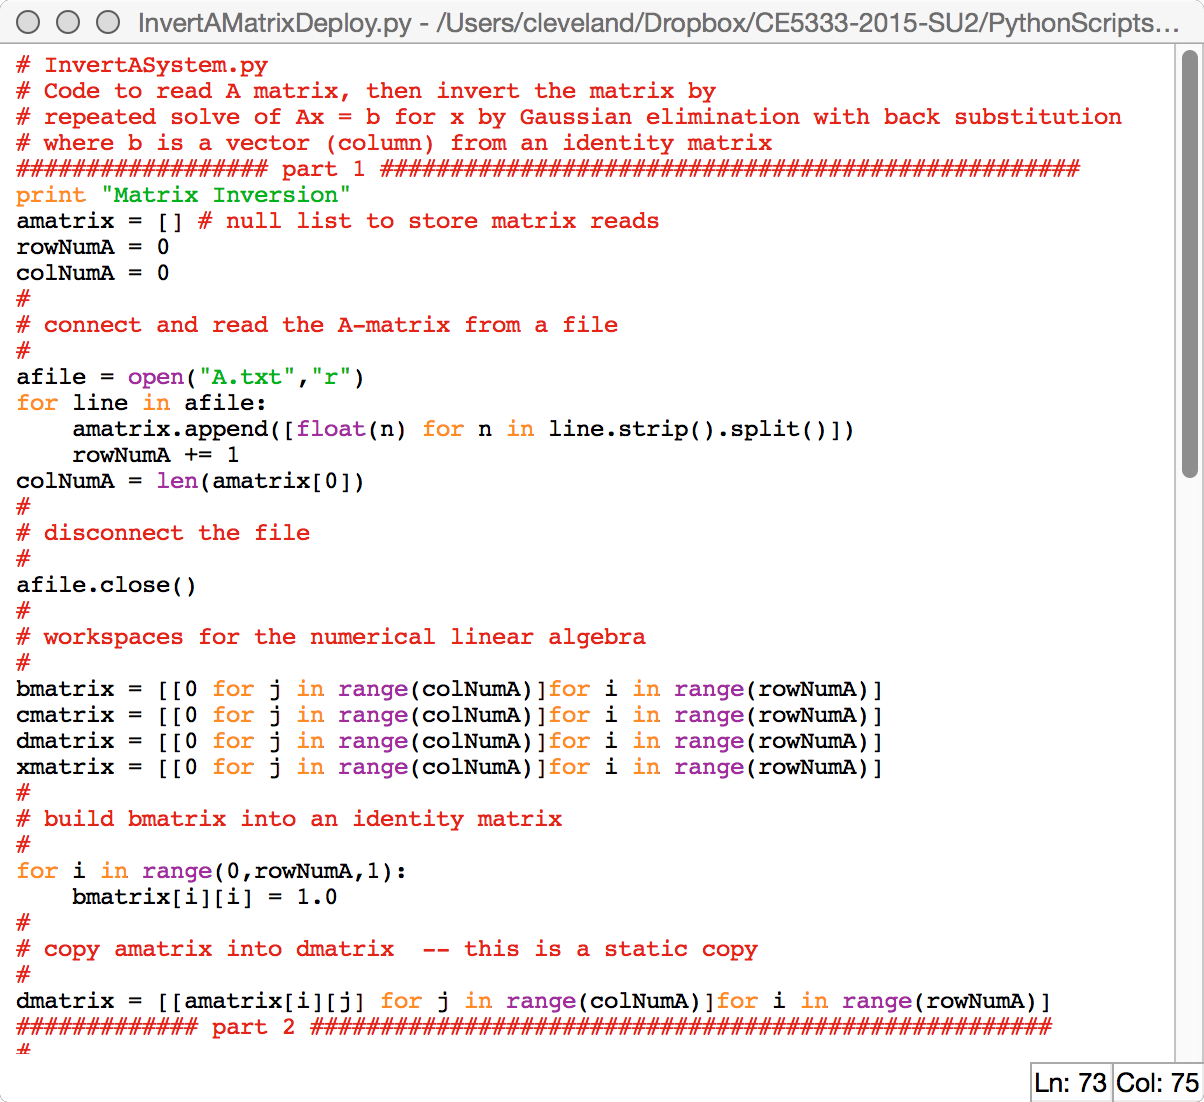
\includegraphics[width=6in]{./9-Matrix/InversionOne.jpg} 
   \caption{Matrix inversion script -- part 1.  Read in the data and set up workspaces.}
   \label{fig:InversionOne}
\end{figure}


\begin{figure}[h!] %  figure placement: here, top, bottom, or page
   \centering
   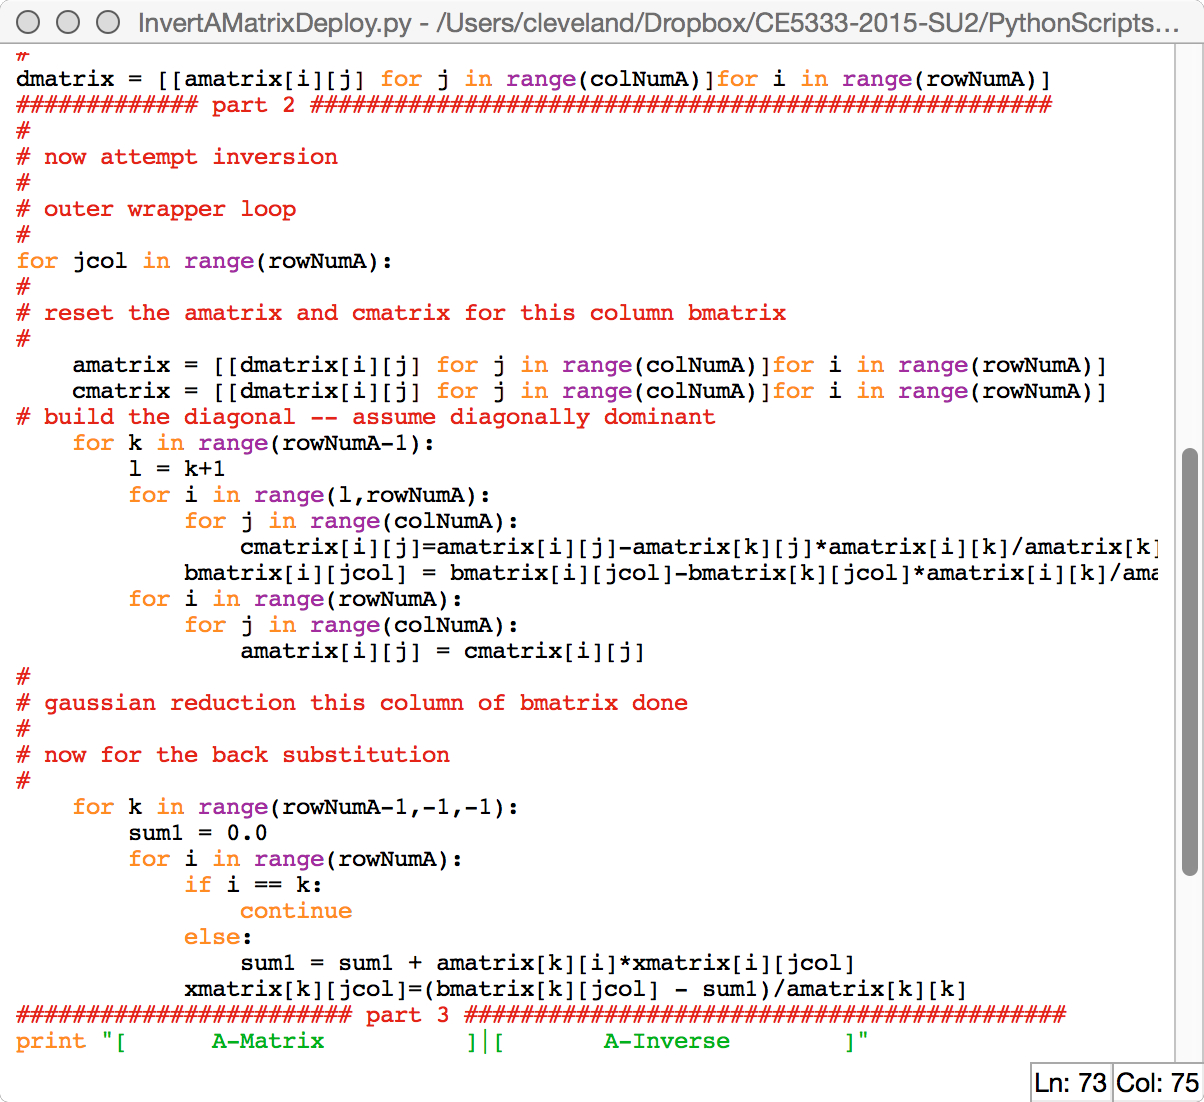
\includegraphics[width=6in]{./9-Matrix/InversionTwo.jpg} 
   \caption{Matrix inversion script -- part 2.  Repeated Gaussian reduction and back-substitution with a changing ring hand side.  The right hand side is a collection of basis vectors that build up an identity matrix.}
   \label{fig:InversionTwo}
\end{figure}

\begin{figure}[h!] %  figure placement: here, top, bottom, or page
   \centering
   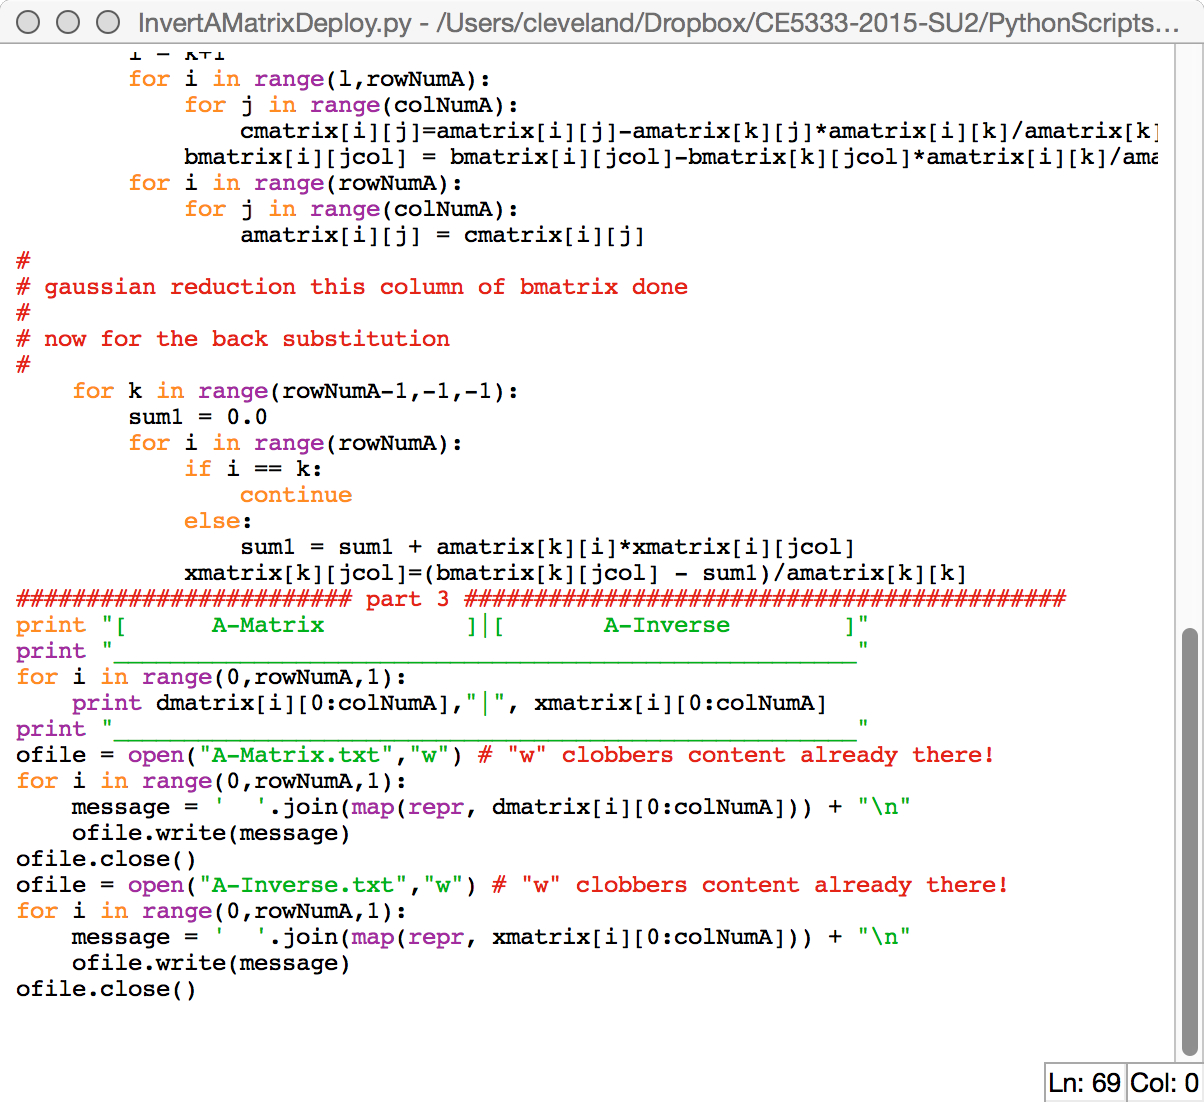
\includegraphics[width=6in]{./9-Matrix/InversionThree.jpg} 
   \caption{Matrix inversion script -- part 3.  Writing the results.}
   \label{fig:InversionThree}
\end{figure}
\clearpage

Figure \ref{fig:InvertedMatrix} is a screen capture of running the script -- as well as showing the output files that are generated.  The figure is really busy, so take time to study it.   The input file, and two output files are shown with the shell output in the background.

\begin{figure}[h!] %  figure placement: here, top, bottom, or page
   \centering
   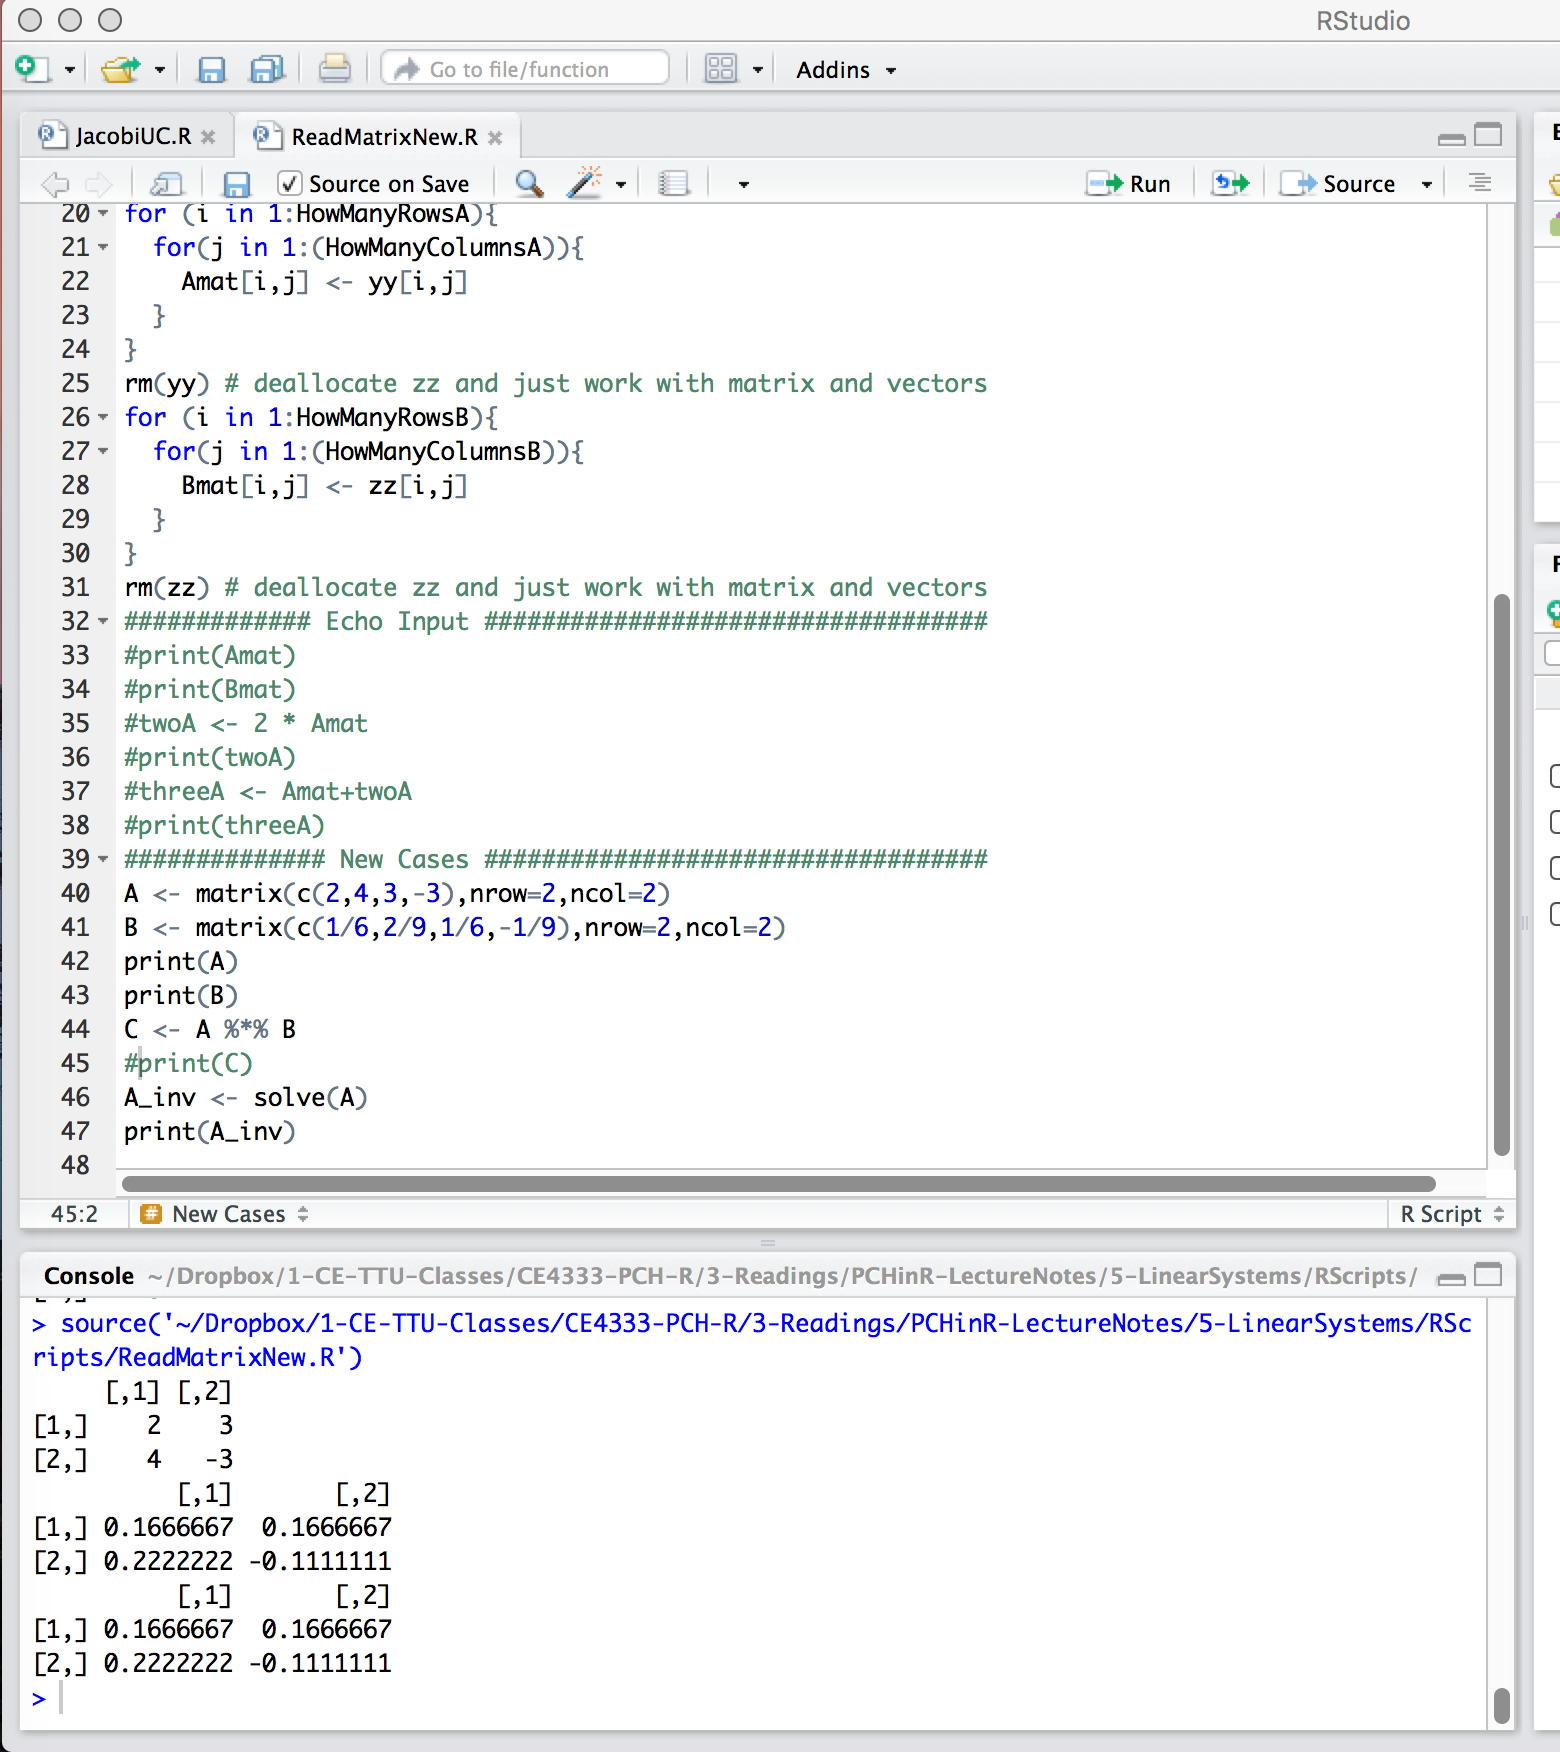
\includegraphics[width=6in]{./9-Matrix/InvertedMatrix.jpg} 
   \caption{The matrix inversion script  showing results of a run and various input and output.}
   \label{fig:InvertedMatrix}
\end{figure}
\clearpage


\subsection{Exercises}
\begin{enumerate}
\item Develop a program to multiply two matrices.  
\begin{enumerate}
\item Apply the program to find $\mathbf{A}\mathbf{x}$ where.
\begin{gather}
\mathbf{A} =
\begin{pmatrix}
4.0 &  1.5 & 0.7 & 1.2 & 0.5 \\
1.0 & 6.0 & 0.9 & 1.4 & 0.7 \\
0.5 & 1.0 & 3.9 & 3.2 & 0.9 \\
0.2 & 2.0 & 0.2 & 7.5 & 1.9  \\
1.7 & 0.9 & 1.2 & 2.3 & 4.9 \\
\end{pmatrix}
~ \mathbf{x} = 
\begin{pmatrix}
0.595194878133 \\
0.507932173989 \\
0.831708392507 \\
0.630365599089 \\ 
1.03737526565 \\
\end{pmatrix}
\end{gather}
\item Use your matrix multiplication program to demonstrate that the inversion example (the 5X5 system above) does indeed produce an inverse matrix.
\item Use the matrix multiplication program again to demonstrate that $\mathbf{x} = \mathbf{A}^{-1} \mathbf{b}$ where
\begin{gather}
\mathbf{A} =
\begin{pmatrix}
4.0 &  1.5 & 0.7 & 1.2 & 0.5 \\
1.0 & 6.0 & 0.9 & 1.4 & 0.7 \\
0.5 & 1.0 & 3.9 & 3.2 & 0.9 \\
0.2 & 2.0 & 0.2 & 7.5 & 1.9  \\
1.7 & 0.9 & 1.2 & 2.3 & 4.9 \\
\end{pmatrix}
~ \mathbf{b} = 
\begin{pmatrix}
5.0 \\
6.0 \\
7.0 \\
8.0 \\ 
9.0 \\
\end{pmatrix}
\end{gather}
\end{enumerate}
\item Develop a program to solve the following linear system of equations
\begin{gather}
\begin{matrix}
2x_1 & ~-~~2x_2 & ~~+3x_3 \\
2x_1 & ~+~~1x_2 & ~~-2x_3 \\
4x_1 & ~-~~1x_2 & ~~-3x_3 \\
\end{matrix}
\begin{matrix}
=~10\\
=~-2\\
=~0\\
\end{matrix}
\end{gather}

\item Develop a program to solve the following linear system of equations\footnote{This is a somewhat tricky problem --- the rows need to be interchanged so that the diagonal is non-zero.  If you use the matrix inverter with the system as presented you will get an error,  but if you rearrange the rows so that the diagonal term is non-zero for each row, then the solver works.  An improved version of the inverter would detect the singular nature and attempt to pivot (swap rows) to generate an investable matrix.  That is left to you to ponder.}
\begin{gather}
\begin{matrix}
0.866x_1 & 0x_2 & -0.5x_3 & 0x_4 & 0x_5 & 0x_6 \\
0.5x_1 & 0x_2 & 0.866x_3 & 0x_4 & 0x_5 & 0x_6 \\
-0.866x_1 & -1x_2 & 0x_3 & -1x_4 & 0x_5 & 0x_6 \\
-0.5x_1 & 0x_2 & 0x_3 & 0x_4 & -1x_5 & 0x_6 \\
-0.5x_1 & 0x_2 & 0x_3 & x_4 & x_5 & x_6 \\
0x_1 & 0x_2 & -0.866x_3 & 0x_4 & 0x_5 & -1x_6 \\
\end{matrix}
\begin{matrix}
=~~~~0\\
=-1000\\
=~~~~0\\
=~~~~0\\
=~~~~0\\
=~~~~0\\
\end{matrix}
\end{gather}

%\item Develop a program to compute the determinant of a matrix --- apply the program to the coefficient matrix in the previous problem.   

\end{enumerate}
\subsubsection{Application Project: Static Truss Analysis}
Figure \ref{fig:StaticTrussSketch} is a simply supported, statically determinate truss with pin connections (zero moment transfer connections).   Find forces in each member for the loading shown.
\begin{figure}[htbp] %  figure placement: here, top, bottom, or page
   \centering
   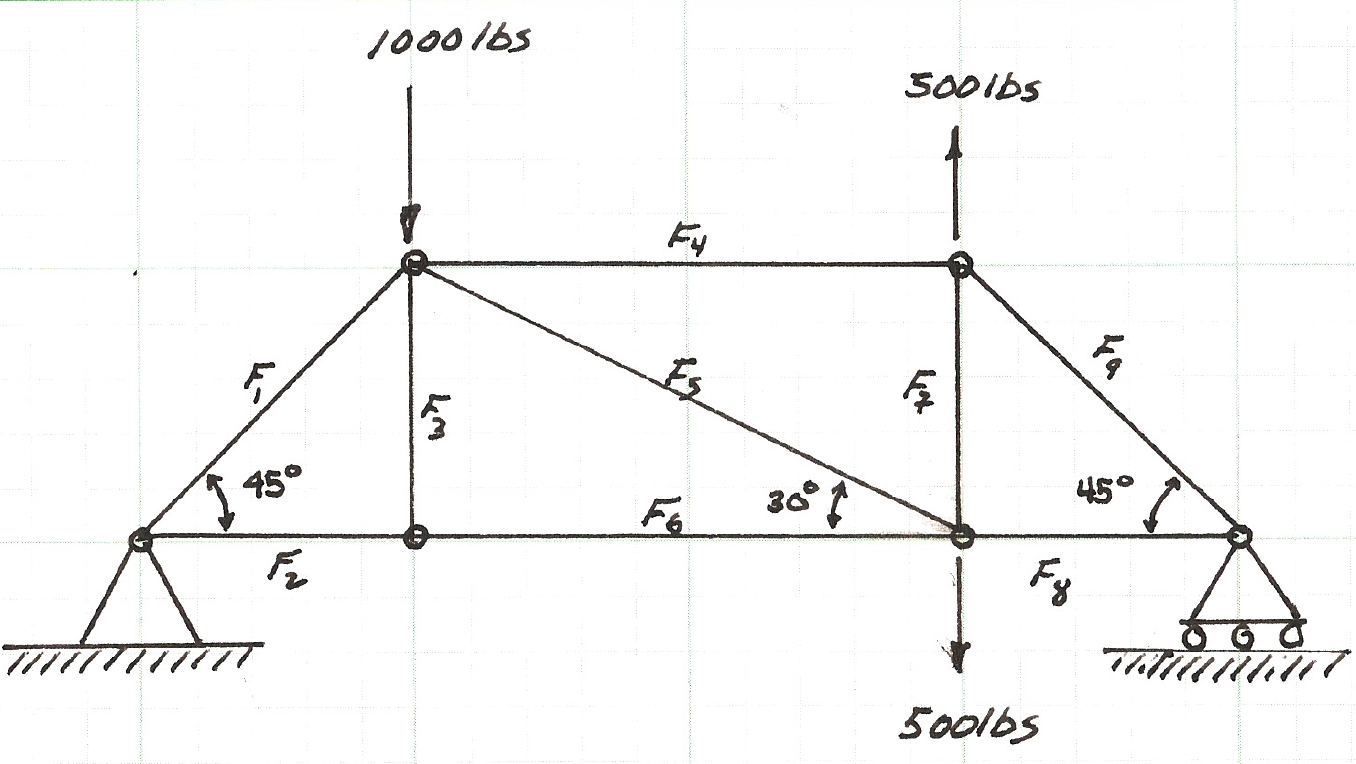
\includegraphics[width=4in]{./9-Matrix/StaticTrussSketch.jpg} 
   \caption{Sketch of simply supported, static truss}
   \label{fig:StaticTrussSketch}
\end{figure}

\textsl{Static Analysis}
Before even contemplating writing/using a program we need to build a mathematical model of the truss and assemble the system of linear equations that result from the model.  So the first step is to sketch a free-body-diagram as in Figure \ref{fig:StaticTrussFBD} and build a node naming convention and force names.

\begin{figure}[h!] %  figure placement: here, top, bottom, or page
   \centering
   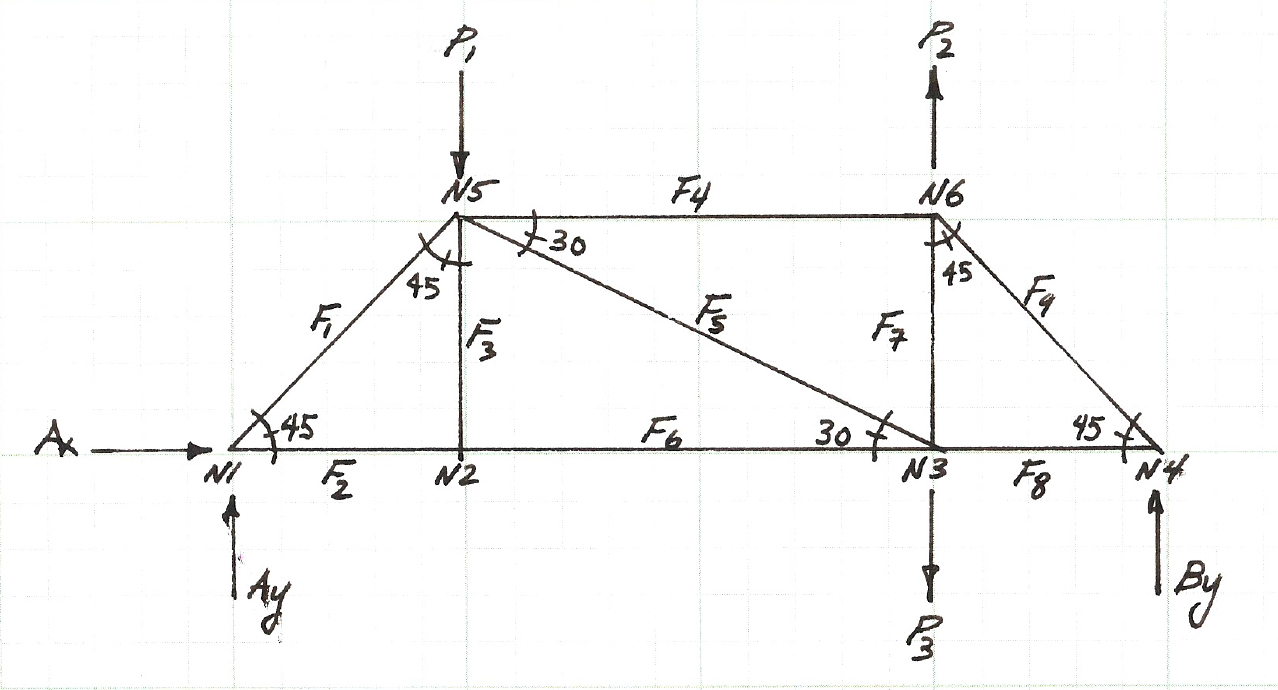
\includegraphics[width=4in]{./9-Matrix/StaticTrussFBD.jpg} 
   \caption{Static truss free-body-diagram showing forces and node naming convention.}
   \label{fig:StaticTrussFBD}
\end{figure}

Next we will write the force balance for each of the six nodes ($N1$-$N6$), which will produce a total of 12 equations in the 12 unknowns (the 9 member forces, and 3 reactions).
\clearpage
Figure \ref{fig:Node1} is the force balance for node $N1$, the two force equations (for the horizontal, $x$, direction and the vertical, $y$, direction) are listed below the figure.
\begin{figure}[h!] %  figure placement: here, top, bottom, or page
   \centering
   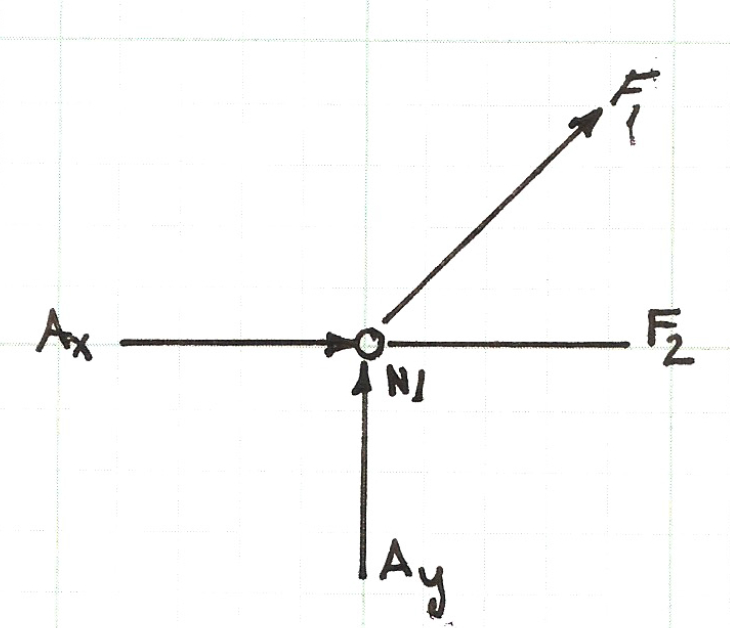
\includegraphics[width=2in]{./9-Matrix/Node1.jpg} 
   \caption{Force diagram at node N1}
   \label{fig:Node1}
\end{figure}

\begin{gather}
\begin{small}
%\mathbf{A} =
\begin{matrix}
\sum F_x = 0 = & +F_1cos(45) & + F_2 &  &  &  &  &  &  & + A_x &  &  & & & \\
\sum F_y = 0 = & +F_1sin(45) &  & &  &  &  &  &  &  &  & + A_y &  &  & \\
\end{matrix}
\end{small}
\label{eqn:Node1Pair}
\end{gather}

Equation \ref{eqn:Node1Pair} is the force balance equation pair for the node.  The $x$ component equation will later be named $N1_x$ to indicate it arises from Node 1, $x$ component equation.   A similar notation convention will also be adopted for the $y$ component equation.  There will be an equation pair for each node.
\begin{figure}[h!] %  figure placement: here, top, bottom, or page
   \centering
   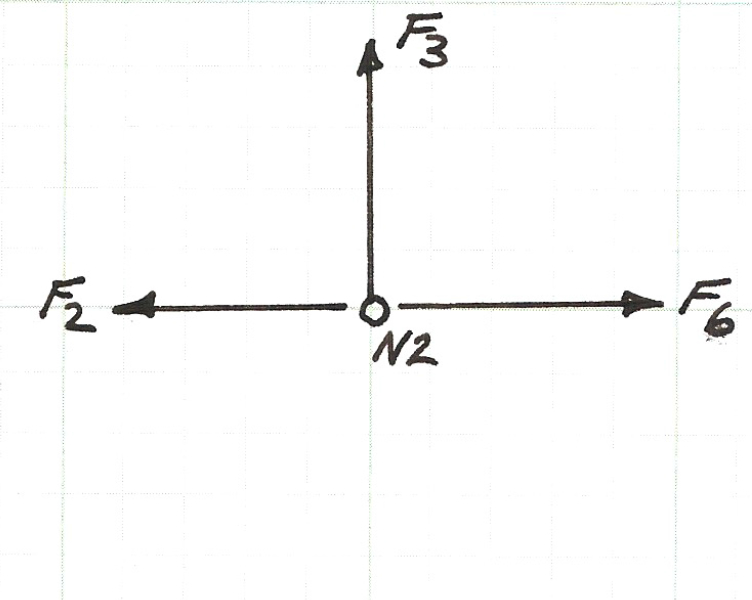
\includegraphics[width=2in]{./9-Matrix/Node2.jpg} 
   \caption{Force diagram at node N2}
   \label{fig:Node2}
\end{figure}

\begin{gather}
\begin{small}
%\mathbf{A} =
\begin{matrix}
\sum F_x = 0 = &  & -F_2 &  &  &  & +F_6 &  &  &  &  &  &  & & \\
\sum F_y = 0 =  &  &  & +F_3 &  &  &  &  &  &  &  &  &  & & \\
\end{matrix}
\end{small}
\label{eqn:Node2Pair}
\end{gather}
Equation \ref{eqn:Node2Pair} is the force balance equation pair for node $N2$.
\clearpage

\begin{figure}[h!] %  figure placement: here, top, bottom, or page
   \centering
   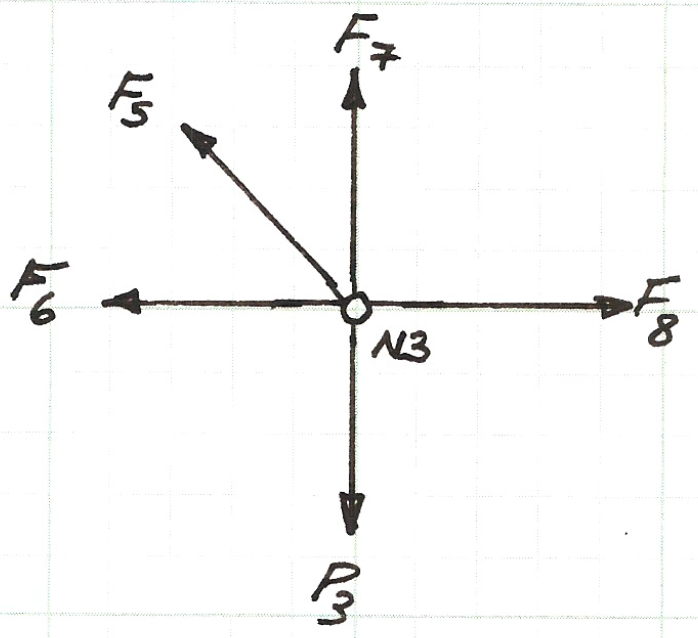
\includegraphics[width=2in]{./9-Matrix/Node3.jpg} 
   \caption{Force diagram at node N3}
   \label{fig:Node3}
\end{figure}

\begin{gather}
\begin{small}
%\mathbf{A} =
\begin{matrix}
\sum F_x = 0 = &  &  &  &  & -F_5cos(30) & -F_6 & & +F_8 &  &  &  &  &  & \\
\sum F_y = 0 =  &  &  &  &  & F_5sin(30) &  & +F_7 &  &  &  &  &  &  & -P_3\\
\end{matrix}
\end{small}
\label{eqn:Node3Pair}
\end{gather}
Equation \ref{eqn:Node3Pair} is the force balance equation pair for node $N3$.

\begin{figure}[h!] %  figure placement: here, top, bottom, or page
   \centering
   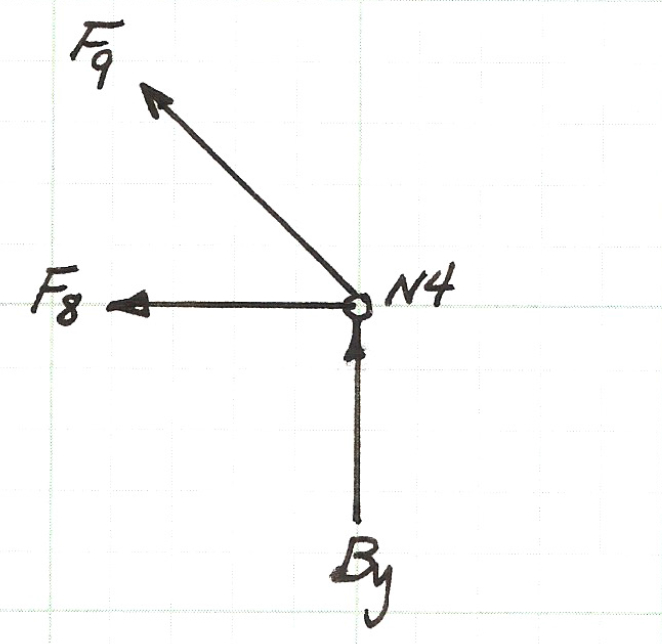
\includegraphics[width=2in]{./9-Matrix/Node4.jpg} 
   \caption{Force diagram at node N4}
   \label{fig:Node4}
\end{figure}

\begin{gather}
\begin{small}
%\mathbf{A} =
\begin{matrix}
\sum F_x = 0 = &  &  &  &  &  &  &  & -F_8 & -F_9cos(45) &  &  &  &  & \\
\sum F_y = 0 =  &  &  &  &  &  &  &  &  & F_9sin(45) &  &  & +B_y  &  & \\
\end{matrix}
\end{small}
\label{eqn:Node4Pair}
\end{gather}
Equation \ref{eqn:Node4Pair} is the force balance equation pair for node $N4$.
\clearpage

\begin{figure}[h!] %  figure placement: here, top, bottom, or page
   \centering
   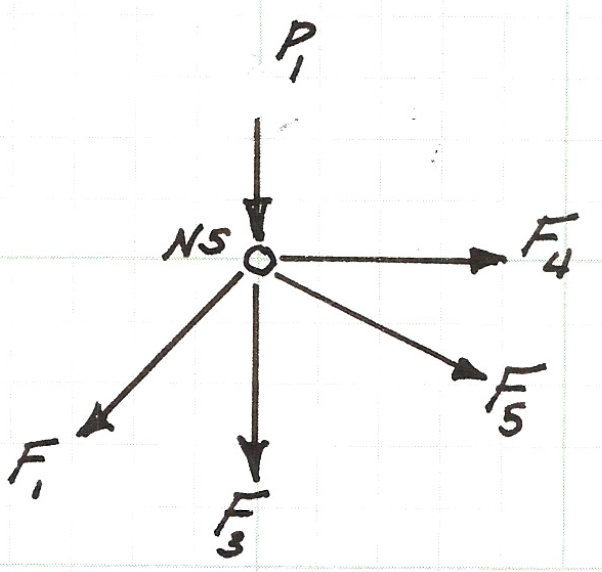
\includegraphics[width=2in]{./9-Matrix/Node5.jpg} 
   \caption{Force diagram at node N5}
   \label{fig:Node5}
\end{figure}

\begin{gather}
\begin{small}
%\mathbf{A} =
\begin{matrix}
\sum F_x = 0 = & -F_1cos(45) &  &   & +F_4 & +F_5cos(30) &  &  &  &  &  &  &  &  & \\
\sum F_y = 0 =  & -F_1sin(45) &  & -F_3 &   & -F_5sin(30) &  &  &  &  &  &  &  &  & -P_1\\
\end{matrix}
\end{small}
\label{eqn:Node5Pair}
\end{gather}
Equation \ref{eqn:Node5Pair} is the force balance equation pair for node $N5$.

\begin{figure}[h!] %  figure placement: here, top, bottom, or page
   \centering
   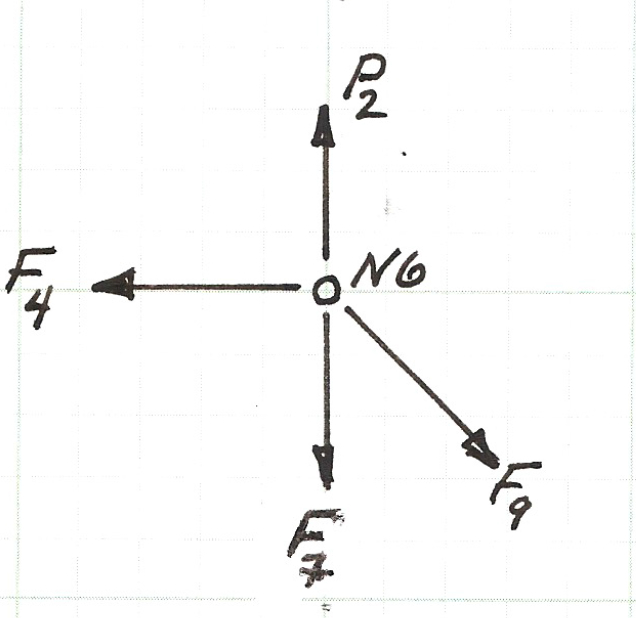
\includegraphics[width=2in]{./9-Matrix/Node6.jpg} 
   \caption{Force diagram at node N6}
   \label{fig:Node6}
\end{figure}
\begin{gather}
\begin{small}
%\mathbf{A} =
\begin{matrix}
\sum F_x = 0 = &  &  &  & -F_4 &  &  &  &  & F_9sin(45) &  &  &  &  & \\
\sum F_y = 0 =  &  &  &  &  &  &  & -1 &  & -F_9cos(45) &  &  &  &  & P_2\\
\end{matrix}
\end{small}
\label{eqn:Node6Pair}
\end{gather}
Equation \ref{eqn:Node6Pair} is the force balance equation pair for node $N6$.
\clearpage

The next step is to gather the equation pairs into a system of linear equations.   We will move the known loads to the right hand side and essentially construct the matrix equation $\mathbf{A}\mathbf{x} = \mathbf{b}$.   Equation \ref{eqn:AugmentTrussMatrix} is a matrix representation of the equation pairs with the forces moved to the right hand side $\mathbf{b} = RHS$. 
\begin{gather}
\begin{small}
%\mathbf{A} =
\begin{pmatrix}
~ & F_1 & F_2 & F_3 & F_4 & F_5 & F_6 & F_7 & F_8 & F_9 & A_x & A_y & B_y & | & RHS\\
\hline
N1_x & 0.707 & 1 & 0 & 0 & 0 & 0 & 0 & 0 & 0 & 1 & 0 & 0 & | & 0\\
N1_y & 0.707 & 0 & 0 & 0 & 0 & 0 & 0 & 0 & 0 & 0 & 1 & 0 & | & 0\\
N2_x & 0 & -1 & 0 & 0 & 0 & 1 & 0 & 0 & 0 & 0 & 0 & 0 & | & 0\\
N2_y & 0 & 0 & 1 & 0 & 0 & 0 & 0 & 0 & 0 & 0 & 0 & 0 & | & 0\\
N3_x & 0 & 0 & 0 & 0 & -0.866 & -1 & 0 & 1 & 0 & 0 & 0 & 0 & | & 0\\
N3_y & 0 & 0 & 0 & 0 & 0.5 & 0 & 1 & 0 & 0 & 0 & 0 & 0 & | & P_3\\
N4_x & 0 & 0 & 0 & 0 & 0 & 0 & 0 & -1 & -0.707 & 0 & 0 & 0 & | & 0\\
N4_y & 0 & 0 & 0 & 0 & 0 & 0 & 0 & 0 & 0.707 & 0 & 0 & 0 & | & 0\\
N5_x & -0.707 & 0 & 0 & 1 & 0.866 & 0 & 0 & 0 & 0 & 0 & 0 & 0 & | & 0\\
N5_y & -0.707 & 0 & -1 & 0 & -0.5 & 0 & 0 & 0 & 0 & 0 & 0 & 0 & | & P_1\\
N6_x & 0 & 0 & 0 & -1 & 0 & 0 & 0 & 0 & 0.707 & 0 & 0 & 0 & | & 0\\
N6_y & 0 & 0 & 0 & 0 & 0 & 0 & -1 & 0 & -0.707 & 0 & 0 &  0 & | & -P_2\\
\end{pmatrix}
\end{small}
\label{eqn:AugmentTrussMatrix}
\end{gather}

In Equation \ref{eqn:AugmentTrussMatrix}, the rows are labeled on the left-most column with their node-related equation name.   Thus each row of the matrix corresponds to an equation derived from a node.   The columns are labeled with their respective unknown force (except the last column, which represents the right-hand-side of the system of linear equations).  Thus the coefficient in each column corresponds to a force in each node equation.   The sign of the coefficient refers to the assumed direction the force acts.   In the analysis all the members were assumed to be in tension (except for the reaction forces).   If a coefficient has a value of zero in a particular row, then than force does no act at the node to which the row corresponds.    

From this representation the transition to the formal vector-matrix representation is straightforward.  Equation \ref{eqn:TrussMatrix}, Equation \ref{eqn:TrussX}, Equation \ref{eqn:TrussRHS} are the $\mathbf{A}$ matrix, the $\mathbf{x}$ vector, and the $\mathbf{b}$ vector, respectively.

Finally, like the last problem in the exercises, the rows need to be re-ordered so the main diagonal contains non-zero values before attempting to solve the linear system.   The remaining project task is to rearrange the rows (by-hand is fine, although writing code to generate an ordering would be a worthy endeavor!), then find the unknown forces using the matrix routines we have already constructed.\footnote{In a later chapter full pivoting will be presented, and with full pivoting this system can be solved without the human having to rearrange rows.}   

One pretty cool feature of this analysis, is we solve for the reactions without needing to know member lengths (no moments).  

\begin{gather}
\begin{small}
\mathbf{A} =
\begin{pmatrix}
0.707 & 1 & 0 & 0 & 0 & 0 & 0 & 0 & 0 & 1 & 0 & 0 \\
0.707 & 0 & 0 & 0 & 0 & 0 & 0 & 0 & 0 & 0 & 1 & 0 \\
0 & -1 & 0 & 0 & 0 & 1 & 0 & 0 & 0 & 0 & 0 & 0 \\
0 & 0 & 1 & 0 & 0 & 0 & 0 & 0 & 0 & 0 & 0 & 0 \\
0 & 0 & 0 & 0 & -0.866 & -1 & 0 & 1 & 0 & 0 & 0 & 0 \\
0 & 0 & 0 & 0 & 0.5 & 0 & 1 & 0 & 0 & 0 & 0 & 0 \\
0 & 0 & 0 & 0 & 0 & 0 & 0 & -1 & -0.707 & 0 & 0 & 0 \\
0 & 0 & 0 & 0 & 0 & 0 & 0 & 0 & 0.707 & 0 & 0 & 0 \\
-0.707 & 0 & 0 & 1 & 0.866 & 0 & 0 & 0 & 0 & 0 & 0 & 0 \\
-0.707 & 0 & -1 & 0 & -0.5 & 0 & 0 & 0 & 0 & 0 & 0 & 0 \\
0 & 0 & 0 & -1 & 0 & 0 & 0 & 0 & 0.707 & 0 & 0 & 0 \\
0 & 0 & 0 & 0 & 0 & 0 & -1 & 0 & -0.707 & 0 & 0 &  0 \\
\end{pmatrix}
\end{small}
\label{eqn:TrussMatrix}
\end{gather}

\begin{gather}
\begin{small}
\mathbf{x} =
\begin{pmatrix}
F_1\\
F_2\\
F_3\\
F_4\\
F_5\\
F_6\\
F_7\\
F_8\\
F_9\\
A_x\\
A_y\\
B_y\\
\end{pmatrix}
\end{small}
\label{eqn:TrussX}
\end{gather}

\begin{gather}
\begin{small}
\mathbf{b} =
\begin{pmatrix}
0\\
0\\
0\\
0\\
0\\
P_3\\
0\\
0\\
0\\
P_1\\
0\\
-P_2\\
\end{pmatrix}
\end{small}
\label{eqn:TrussRHS}
\end{gather}

